\documentclass[12pt,oneside]{paper}

\usepackage{listings}
\renewcommand{\lstlistingname}{saucecode}

\lstset{%
  language={C},
  basicstyle={\small},%
  identifierstyle={\small},%
  commentstyle={\small\itshape},%
  keywordstyle={\small\bfseries},%
  ndkeywordstyle={\small},%
  stringstyle={\small\ttfamily},
  frame={tb},
  breaklines=true,
  columns=[l]{fullflexible},%
  numbers=left,%
  xrightmargin=0zw,%
  xleftmargin=3zw,%
  numberstyle={\scriptsize},%
  stepnumber=1,
  numbersep=1zw,%
  lineskip=-0.5ex%
}



% タイトル
\title{1軸レーザー距離センサを用いたQudad Rotorの周辺認識についての研究}
\author{高倉啓祐・中野晋}

\begin{document}
% 行間
\setlength{\baselineskip}{9truemm}

%文字間
\kanjiskip=.53zw plus 3pt minus 3pt
\xkanjiskip=.53zw plus 3pt minus 3pt

% 目次
\tableofcontents
%\newpage

% 本文
\chapter{はじめに}


\section{研究の背景}
近年は,マルチコプターは,農業,空撮,物資配達,救助といった様々な場面で用いられるようになってきた.遠隔操作が可能で,複数のプロペラや翼を搭載した機体である.現代において更なる技術革新と汎用性が求められている.


\section{研究の目的}
本研究室では,マルチコプター通称ドローンを設計から一貫し製作を行ってきた.これまでの研究目標としてきた校内を自律飛行案内するという目標を掲げ活動を行ってきた.中間目標としていた全日本飛行ロボットコンテストに出場し見事に優勝を飾ったが,いくつかの課題も残った.具体的に大会でのミッションとなっていた自動離着陸や,自動八の字飛行ができなかった.また,CFRPを用いたフレームにおいても大会規定であった機体重量に対し,自動飛行用のためのセンサーなどを搭載していた場合,重量規定を超えてしまっていた.そのためより軽く合成のあるフレーム製作が最も重要であり必要不可欠であると考えられた.平面積層のCFRPフレームに対し,より軽量で剛性のあるフレーム製作を目的とする.そのためこれまでの平面積層ではなく,立体構造のフレーム製作を行うこととした.


\begin{figure}[htbp]
  \begin{center}
    \includegraphics[width=120mm]{img/1.JPG}
    \end{center}
  \caption{カーボンフレームのマルチコプター}
 \label{fig:robot}
\end{figure}


\section{本論文の構成}
1章では,本研究の背景と簡略化した概要を示す.また,研究室での自立飛行マルチコプター製作においての自身の役割について述べる,全日本学生飛行ロボットコンテストについて述べる.3章では平面積層フレームの製作工程について述べる.4章では立体積層フレームについて述べる.5章では平面積層と立体積層フレームにおいての強度曲げ試験,および結果について述べる.6章ではフレーム製作についてのまとめを示す.


\chapter{全日本学生飛行ロボットコンテスト}
\section{飛行ロボットコンテストについて}
本研究室では,一貫したマルチコプター製作の中間目標として全日本学生室内飛行ロボットコンテストマルチコプター部門に出場した.
全日本学生室内飛行ロボットコンテストは,室内で飛行する航空機型ロボットによる競技で,マルチコプター部門は,「ドローン」と呼ばれることが多い,複数の回転翼をもつ機体(マルチコプター)で出場します.
同部門のミッションは,ヘリポートから飛行を開始し,ミッションエリアにて各ミッションを完了したのち,ヘリポートに帰還する.


\begin{figure}[htbp]
  \begin{center}
    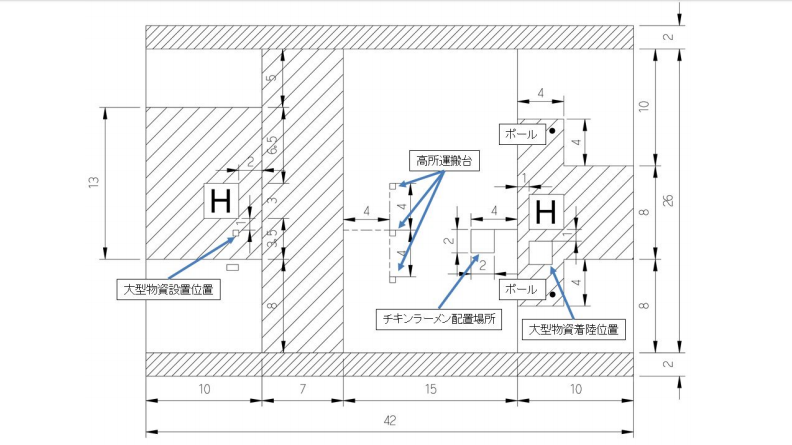
\includegraphics[width=150mm]{img/17.png}
    \end{center}
  \caption{飛行協議エリア}
 \label{fig:robot}

\end{figure}\begin{figure}[htbp]
  \begin{center}
    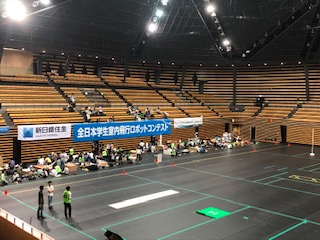
\includegraphics[width=120mm]{img/20.JPG}
    \end{center}
  \caption{大会会場}
 \label{fig:robot}
\end{figure}

\section{大会結果}
今年の予選のミッションは,離陸して高所から物資(チキンラーメン)を正解の高所運搬台に運び,運んだチキンラーメンの数で点数を競い,この,ミッションをクリアすれば「8の字飛行」にチャレンジし,速度や性能を競う.
決勝では,大型の物資運搬にチャレンジし,離着陸エリアからぬいぐるみを結び付けて離陸して,着陸位置にぬいぐるみを静止させ.
接続を保ったままヘリポートに機体を着陸させる.予選と決勝を通じて全てのチャレンジに成功し満点を獲得した.
また,これまでマルチコプター部門には,2回エントリーして2回とも書類審査を通過できず3度目の挑戦で優勝をすることができた.

\begin{figure}[htbp]
  \begin{center}
    \includegraphics[width=120mm]{img/2.JPG}
    \end{center}
  \caption{大会出場機体}
 \label{fig:robot}
\end{figure}

\chapter{平面フレームの製作工程について}

平面フレームを成型するにための型は,ベニヤ板を切り抜いた木枠を用いて製作を行った.

\section{木型の設計}
型の設計は3DCADを用いて行った.平面積層用の木枠は,ベニヤ板をレーザー加工機を用いて切り抜き,制作を行った.雄型,雌型をそれぞれ設計を行った.

\begin{figure}[htbp]
  \begin{center}
    \includegraphics[width=120mm]{img/3.JPG}
    \end{center}
  \caption{フレームの3Dモデル}
 \label{fig:robot}
\end{figure}

\section{レーザー加工機でのカーボンクロスの切り出し}
カーボンクロスをレーザー加工機を用いて切り出す.レーザー加工機を使用する以前は,ハサミで切って切り出していた.しかしカーボンクロスの繊維が細かく,ささくれてしまい積層が困難だった.レーザー加工を行うことで,縁が溶着硬化することができるため積層が綺麗に行うことができる.

\begin{figure}[htbp]
  \begin{center}
    \includegraphics[width=120mm]{img/5.JPG}
    \end{center}
  \caption{切り出されるカーボンクロス}
 \label{fig:robot}
\end{figure}


\section{木型への離型剤吹付け作業}
カーボンクロスの積層には,硬化させるためのエポキシ樹脂を用いる.そのため硬化後に離型を容易にするために離型剤を用いる.平面フレーム用の木型には,枠の縁などに塗りやすいようにスプレー式を用いた.

\begin{figure}[htbp]
  \begin{center}
    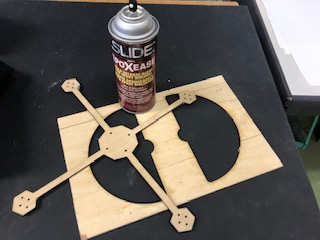
\includegraphics[width=120mm]{img/18.JPG}
    \end{center}
  \caption{離型剤の吹き付けた型}
 \label{fig:robot}
\end{figure}

\section{積層作業}
平面積層においては切り出されたカーボンクロスを枠に合わせ,1枚重ねるごとにエポキシ樹脂を塗り重ね繰り返し行う.重ねる枚数が増えてゆくにつれ塗る硬化剤の量を減らしてゆく.

\begin{figure}[htbp]
  \begin{center}
    \includegraphics[width=120mm]{img/7.JPG}
    \end{center}
  \caption{積層作業}
 \label{fig:robot}
\end{figure}

\section{仕上げ作業}
24時間以上が経過し完全に硬化したフレームは,やすり掛けバリ取りを行い完成となる.

\begin{figure}[htbp]
  \begin{center}
    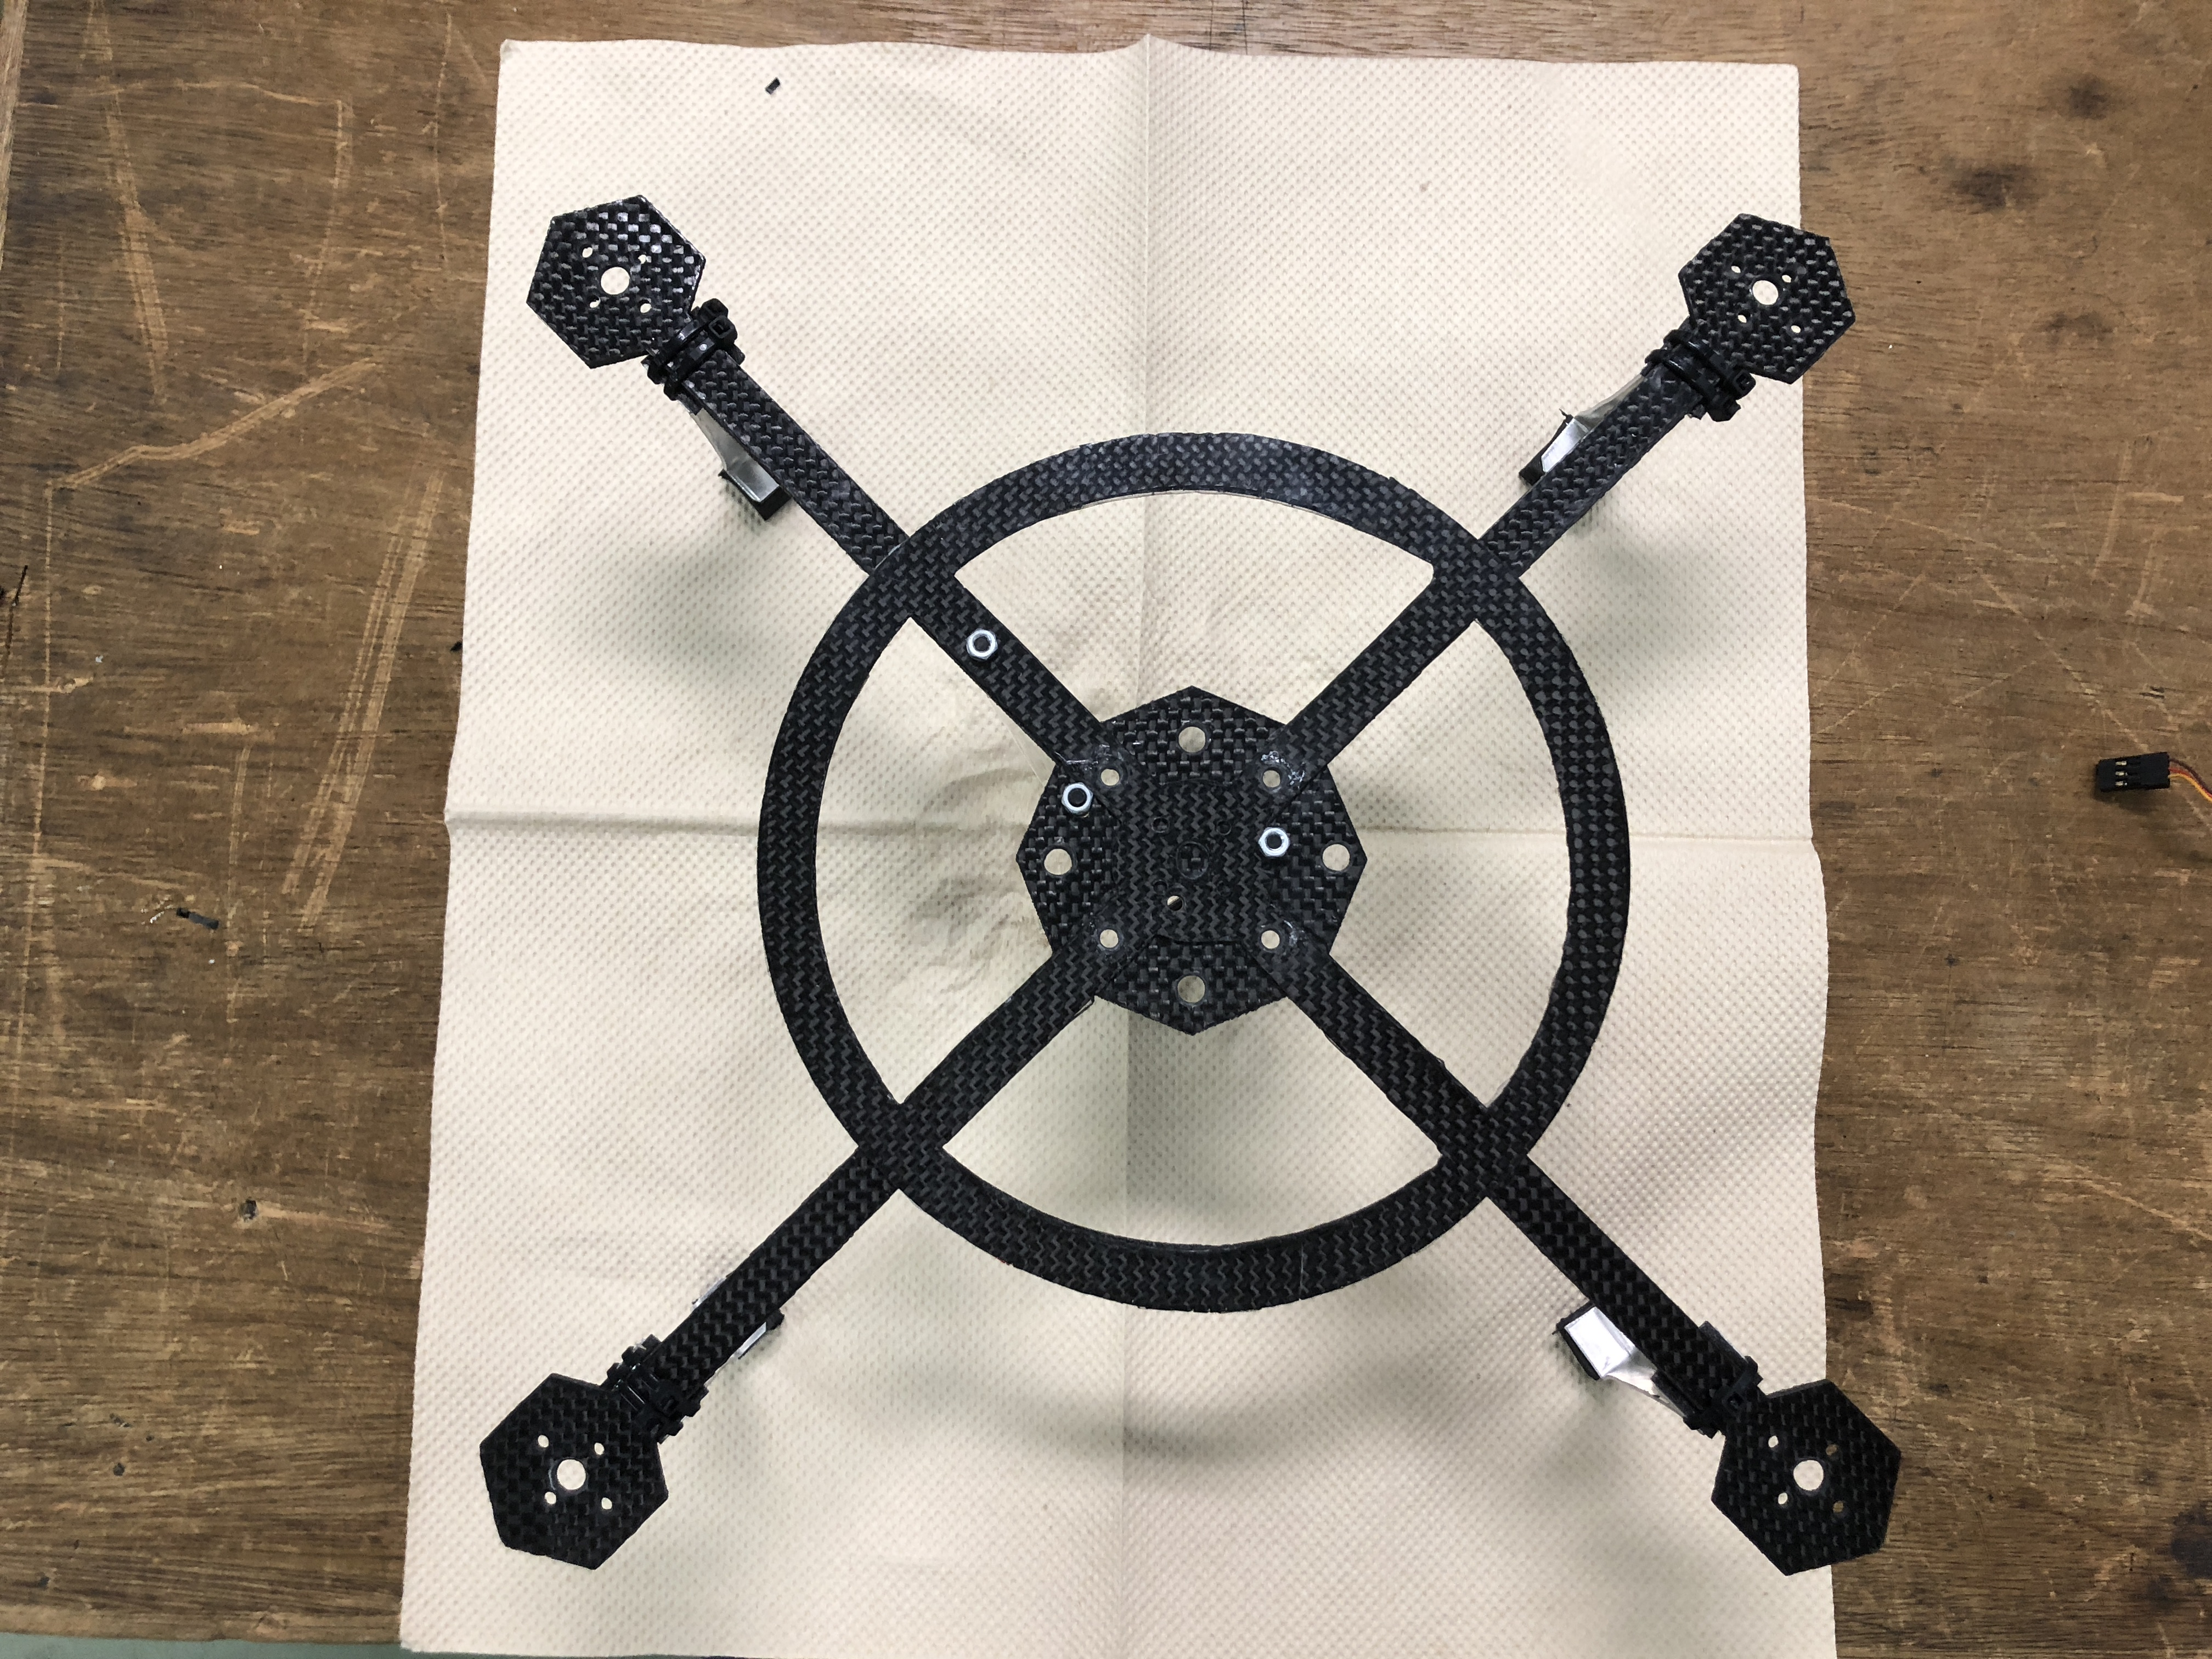
\includegraphics[width=120mm]{img/21.JPG}
    \end{center}
  \caption{完成したフレーム}
 \label{fig:robot}
\end{figure}

\section{平面フレーム製作過程においてのまとめ}
平面フレーム製作において積層硬化後,離型にエポキシ樹脂用スプレー型離型剤とポリプロピレンフィルムを用いた,どちらも容易に離型することはできたが,離型後の表面状態が異なった,スプレー型の専用のモノを使った場合,表面はつやがないマットな仕上がりとなった,しかし,散布する量にむらがあったり,量が多くなりすぎると表面に固着してしまい仕上がり面が綺麗にならないことがあった,それに対しフィルムを用いた場合は,仕上がり面は光沢となり,量による影響も全くないため表面積層においてはポリプロピレンフィルムを用いることが最適である,また平面積層において機体の足部分を,板金で湾曲させた板を用いて立体積層も行った.しかし湾曲部に角がついてしまい着陸時の衝撃ですぐに破損してしまい,平面での立体積層は困難であった.

\begin{figure}[htbp]
  \begin{center}
    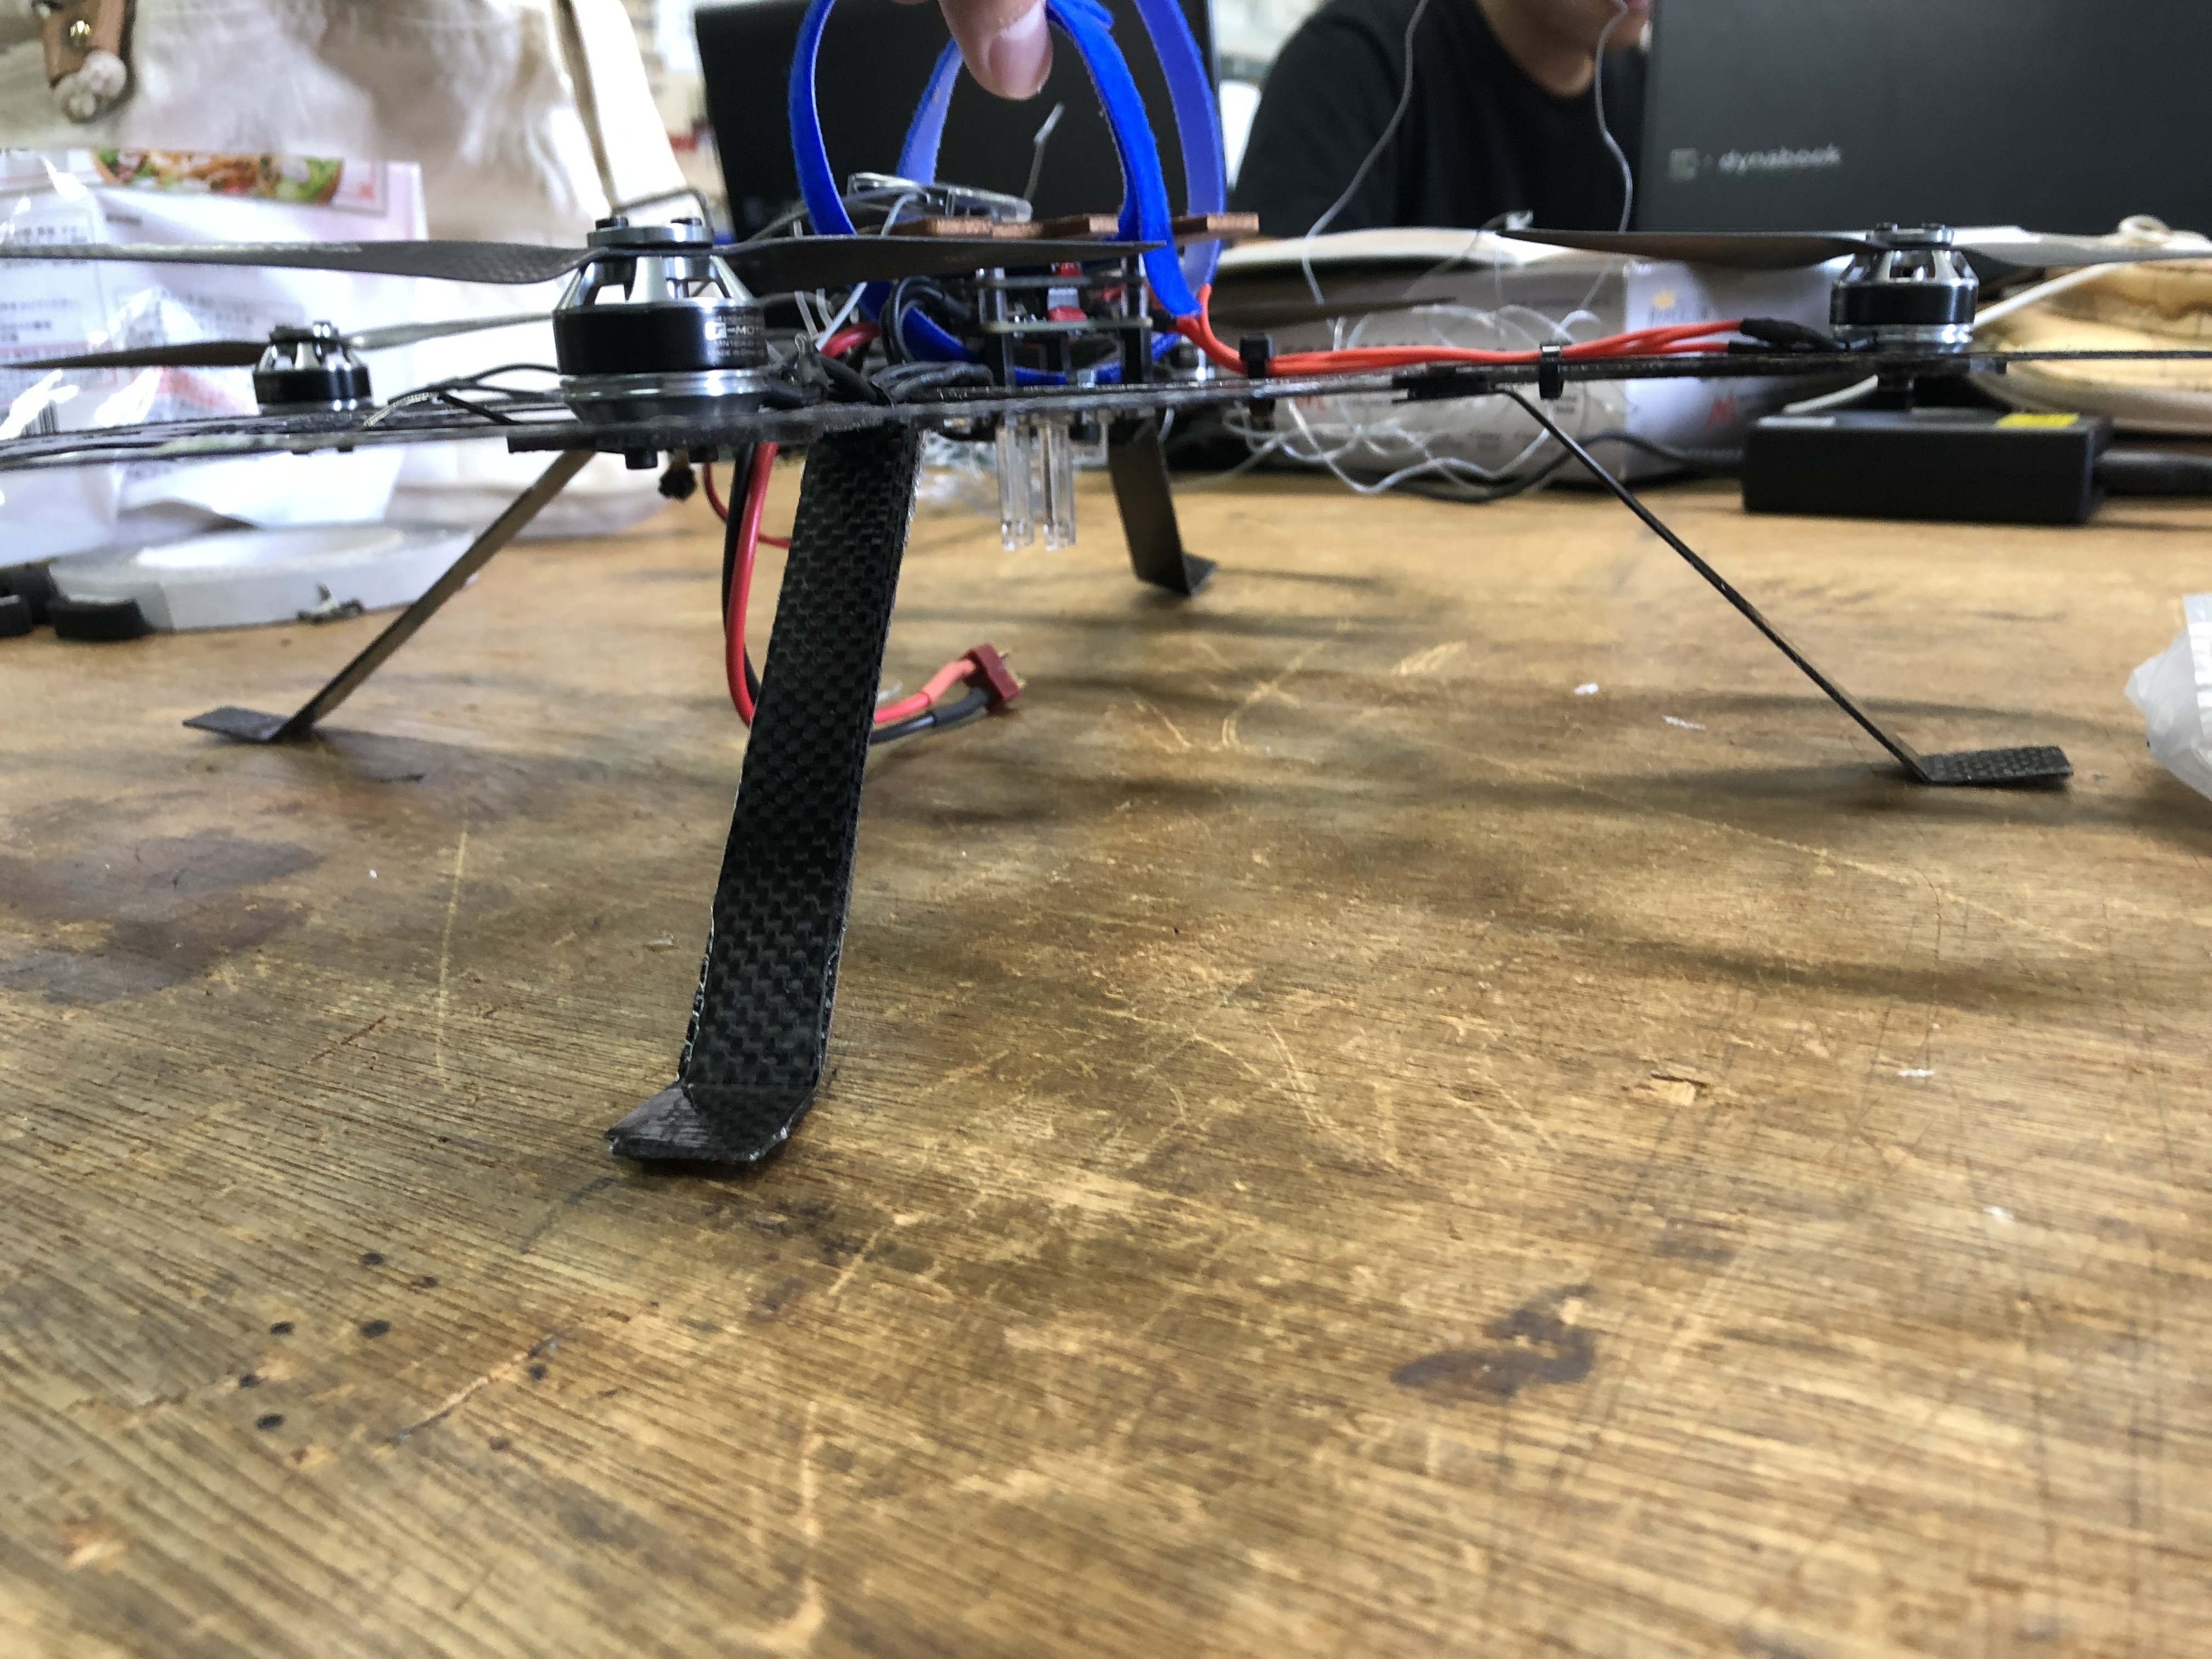
\includegraphics[width=120mm]{img/24.JPG}
    \end{center}
  \caption{平面積層で製作した足}
 \label{fig:robot}
\end{figure}





\chapter{立体積層フレームの製作工程について}
立体フレームを成型するための型は,3DCADにて設計を行い3Dプリンターを用いて制作を行った.

\begin{figure}[htbp]
  \begin{center}
    \includegraphics[width=120mm]{img/6.JPG}
    \end{center}
  \caption{立体フレームの3Dモデル}
 \label{fig:robot}
\end{figure}

\section{プリンターでの立体型造形}
3Dプリンターでの造形には,各型につきそれぞれ6時間から7時間を要した.立体型は雄型,雌型をそれぞれの設計を行った.平面用の木枠は一体型に対し,立体フレーム用の型は大きさの関係上,造形時のプリンターのテーブルに収まらないため二つのパーツに分けて設計をした.積層時に連結するための突起部分も設計されている.また,造形時プリンターのノズルからの樹脂の射出温度と空冷時の室内温度の温度差が大きくなってしまう場合があった.その結果,反りが発生してしまい造形途中でクラックが入ったり,土台がテーブルから浮いてしまうなど,全体のゆがみの原因となってしまった.そのための土台の表面積を増加させ,テーブルにはのりを付着させそれらの防止をする工夫を施した.

\begin{figure}[htbp]
  \begin{center}
    \includegraphics[width=120mm]{img/8.JPG}
    \end{center}
  \caption{造形された型}
 \label{fig:robot}
\end{figure}

\begin{figure}[htbp]
  \begin{center}
    \includegraphics[width=120mm]{img/9.JPG}
    \end{center}
  \caption{型の連結部分}
 \label{fig:robot}
\end{figure}

\section{立体型への離型剤塗り付け作業}
立体フレーム用の型には離型剤として,車用のワックスを利用した.むらができてしまうと離型が困難になってしまうため,ワックスは厚めにぬりこんだ.また圧縮用のポリ袋にはくっつかず容易に離型することができる.

\begin{figure}[htbp]
  \begin{center}
    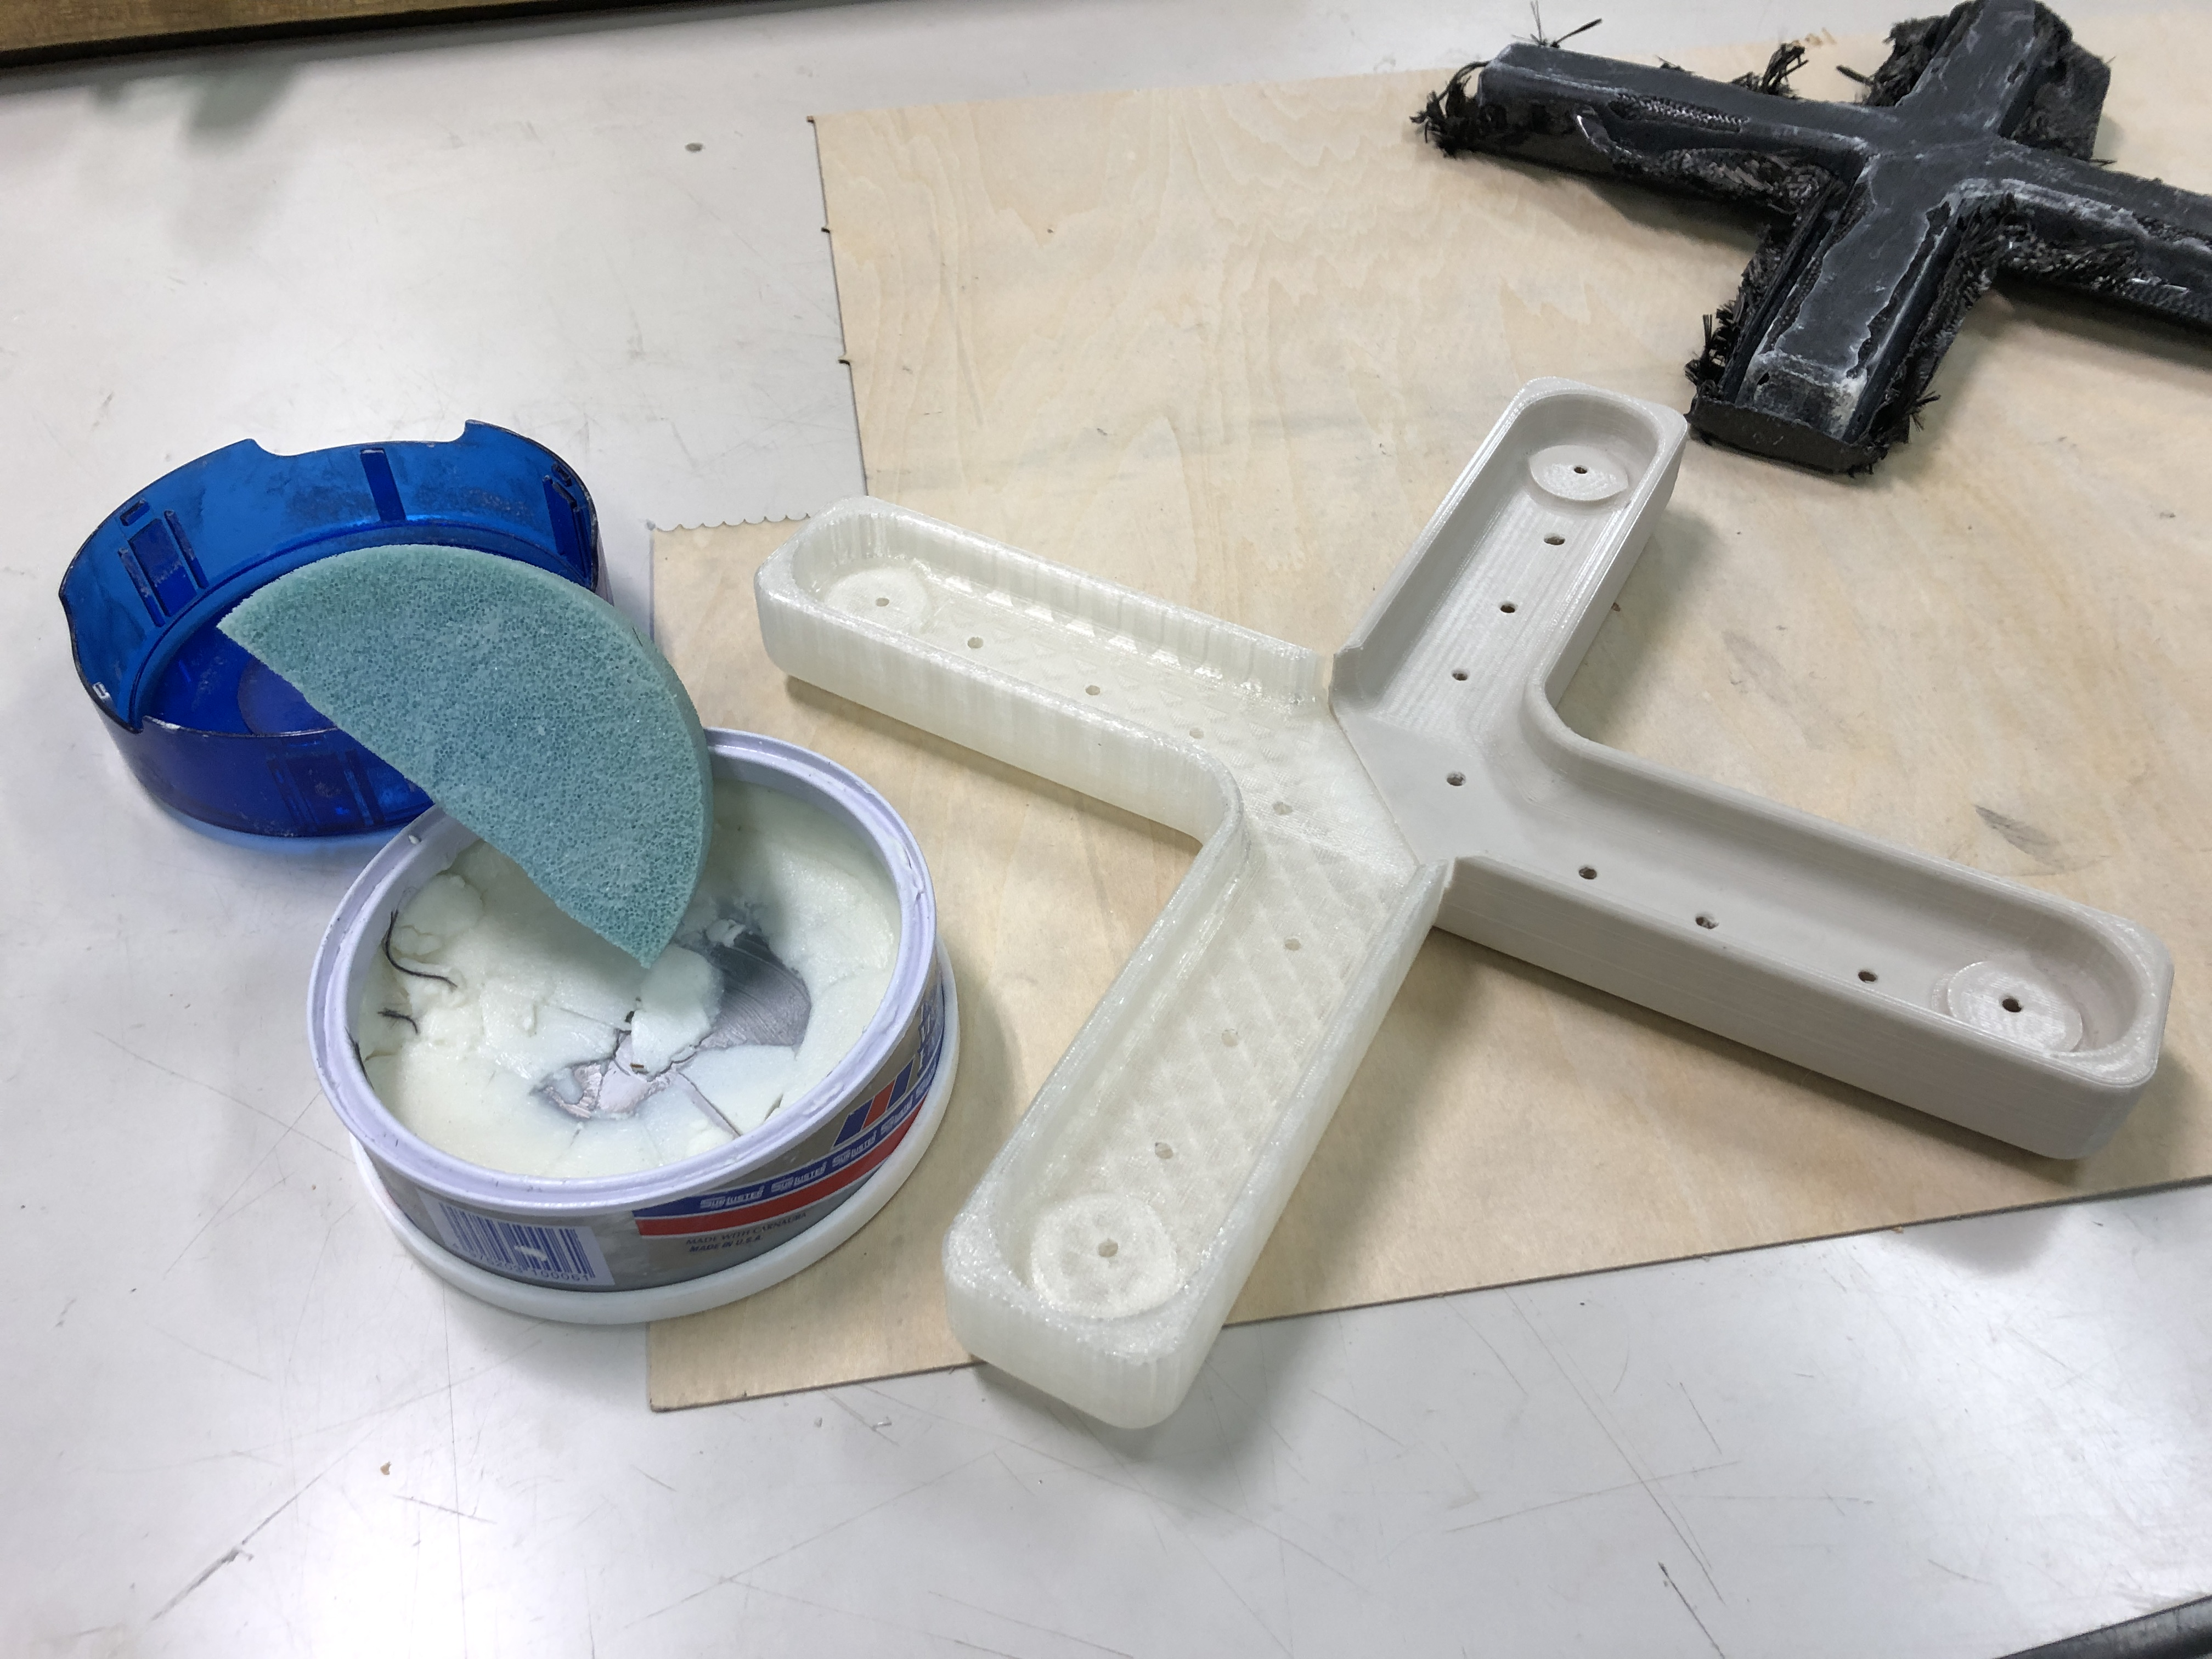
\includegraphics[width=120mm]{img/10.JPG}
    \end{center}
  \caption{ワックスの塗り付け}
 \label{fig:robot}
\end{figure}



\section{積層作業}
離型剤を塗った型にカーボンシートを被せ積層を行っていく.この際に一枚をフレームの形に多い壁せていくのはしわができてしまったりと困難なため,四分割にして行った.型内部の縁に沿って折り目をつけていき,エポキシ樹脂を刷毛で塗っていく.二枚目以降も同様に積層作業を行い,隙間やエッジ部分のしわを極力少なくしてゆく.またカーボンシート枚数を重ねるごとにエポキシ樹脂の量を減少させていく.

\begin{figure}[htbp]
  \begin{center}
    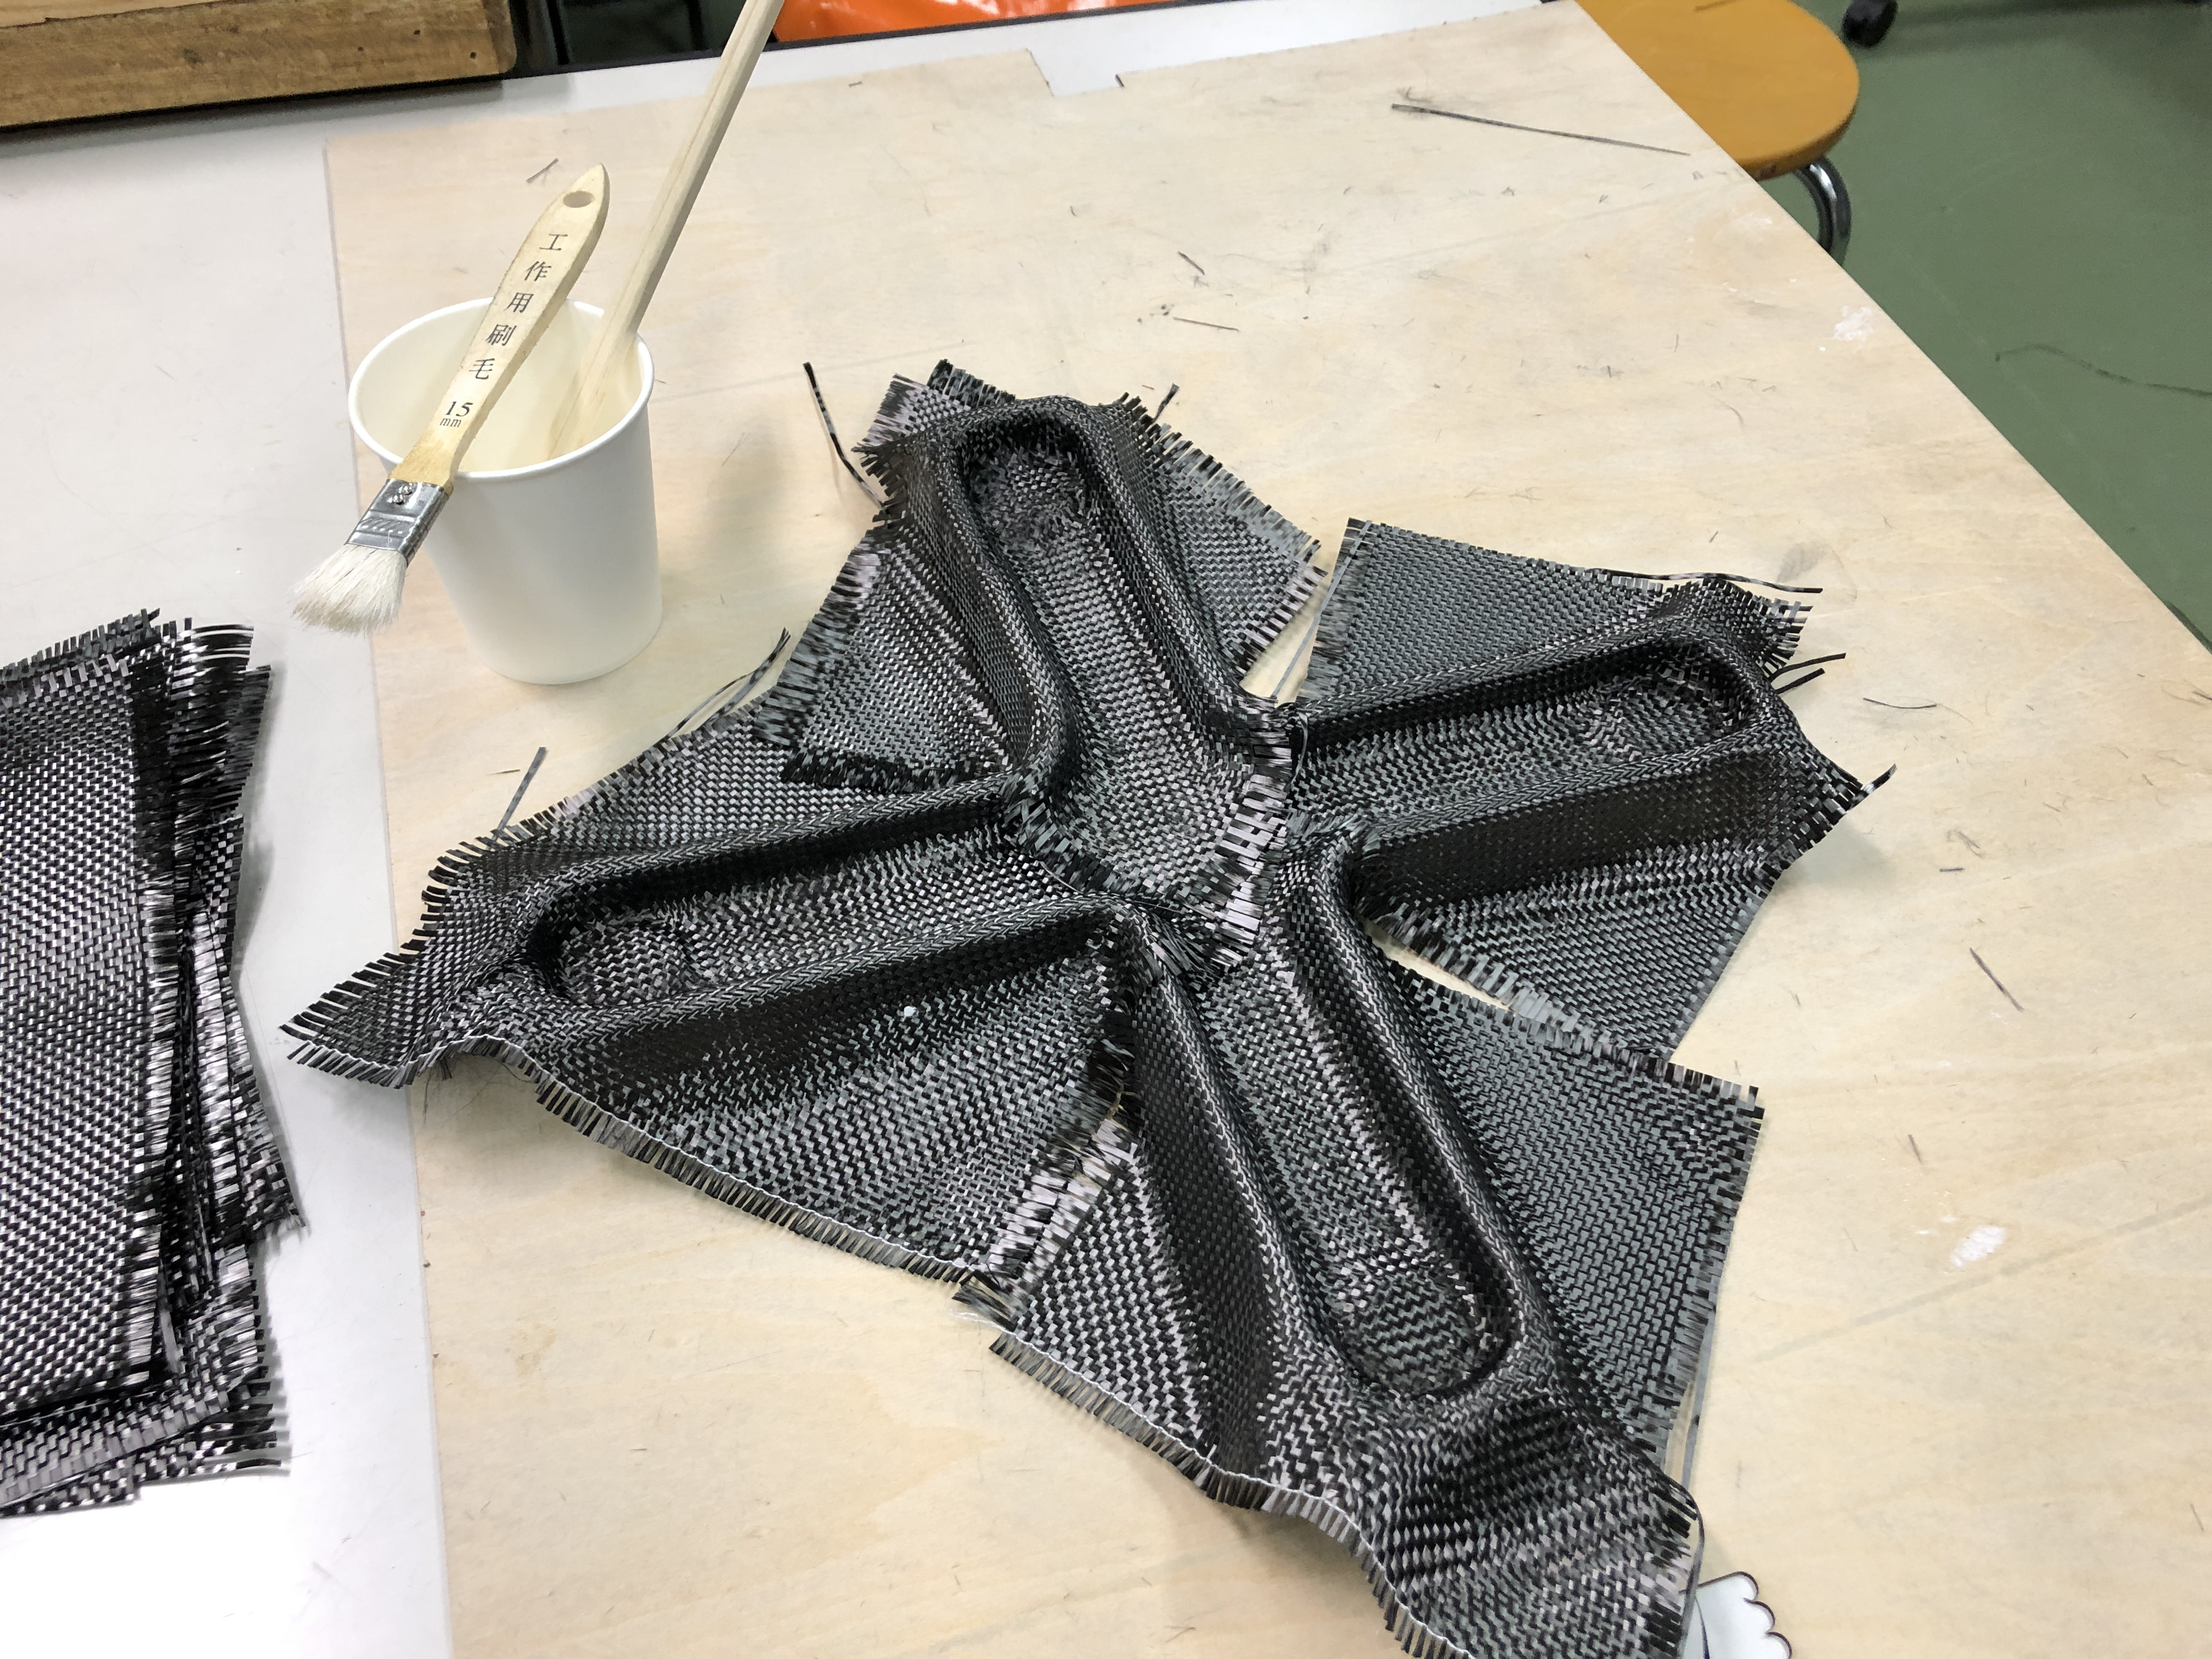
\includegraphics[width=120mm]{img/11.JPG}
    \end{center}
  \caption{四分割された}
 \label{fig:robot}
\end{figure}

\begin{figure}[htbp]
  \begin{center}
    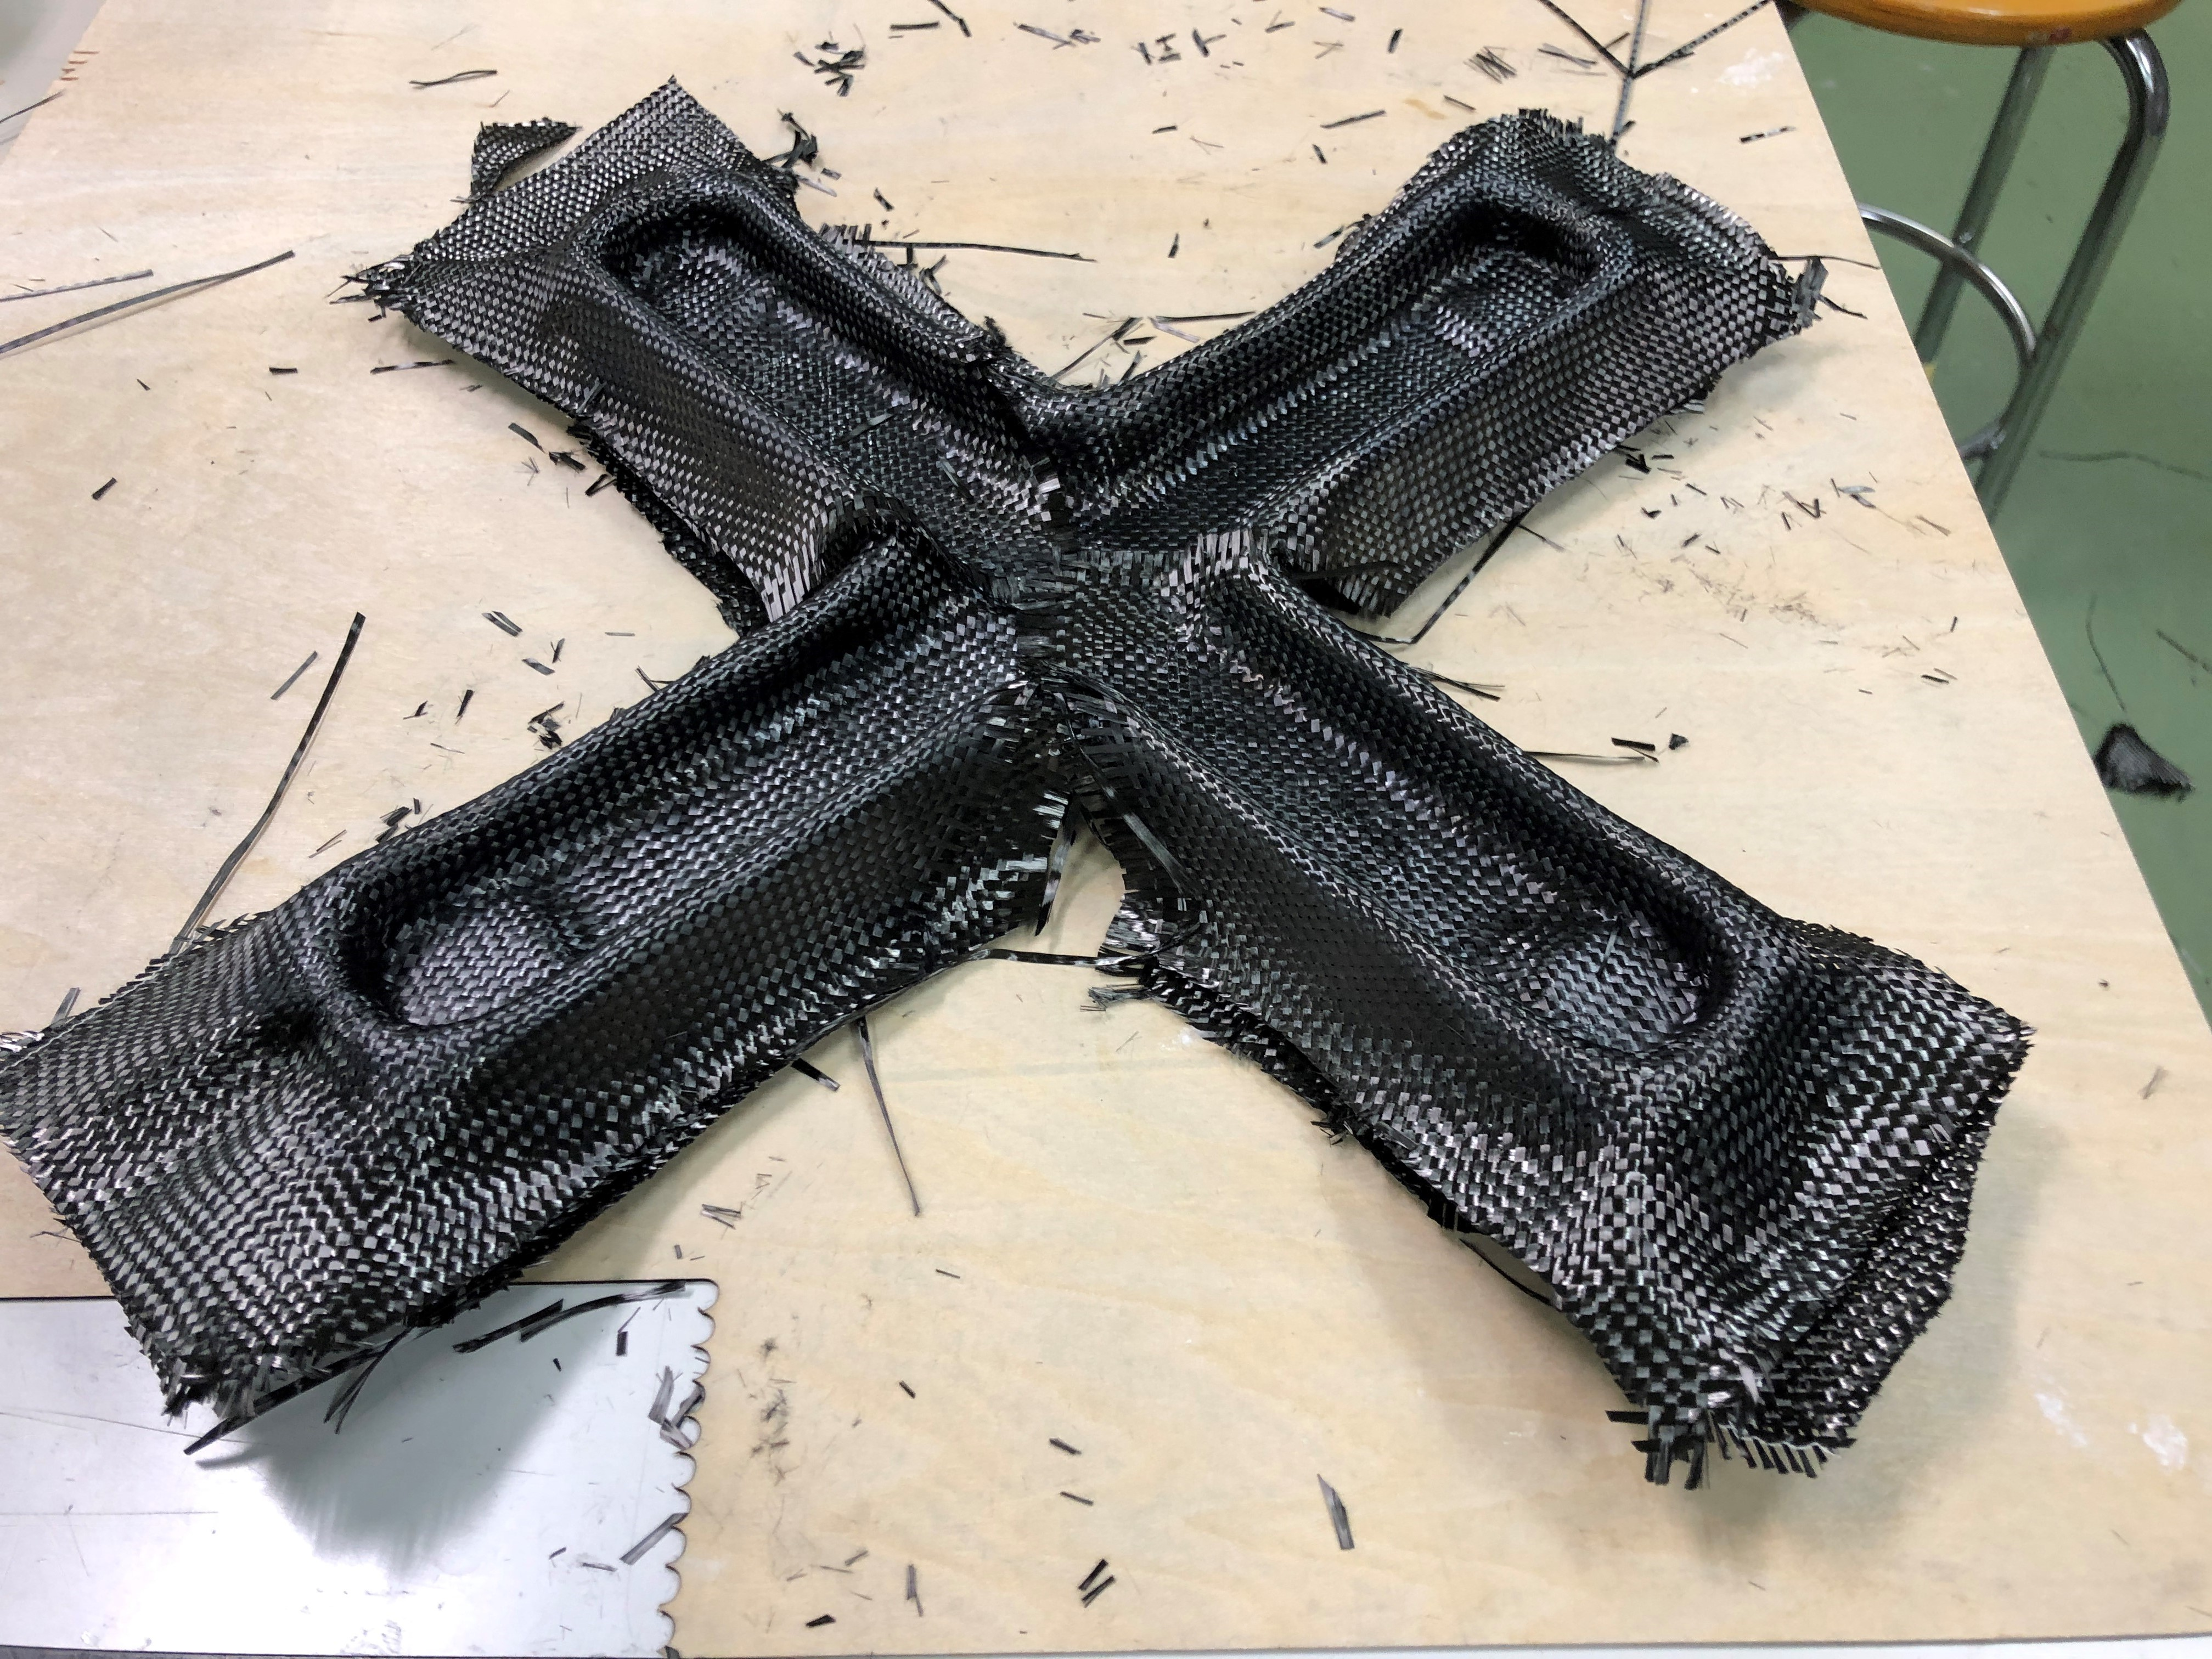
\includegraphics[width=120mm]{img/12.JPG}
    \end{center}
  \caption{硬化剤を塗られ積層されたカーボンシート}
 \label{fig:robot}
\end{figure}

\section{真空引き作業}
圧縮作業には,吸引機として掃除機とビニールポリ袋を用いて作業行った.積層作業を終えたものをビニールポリ袋に入れる.その後吸引のためのノズルを通す部分以外をアイロンで温め溶着させる.その後掃除機で圧縮作業を行っていく.圧縮の際に一気に空気を抜いていくのではなく,徐々に空気量を調整していきながらポリ袋を型の形に添わせながら空気を抜いてゆく.また型の角がポリ袋を傷つけないかを気を付けながら完全に空気を抜いていく.最終的にノズルを抜いていき,すべてを抜ききる手前でアイロンで溶着をさせ圧縮作業が完了する.

\begin{figure}[htbp]
  \begin{center}
    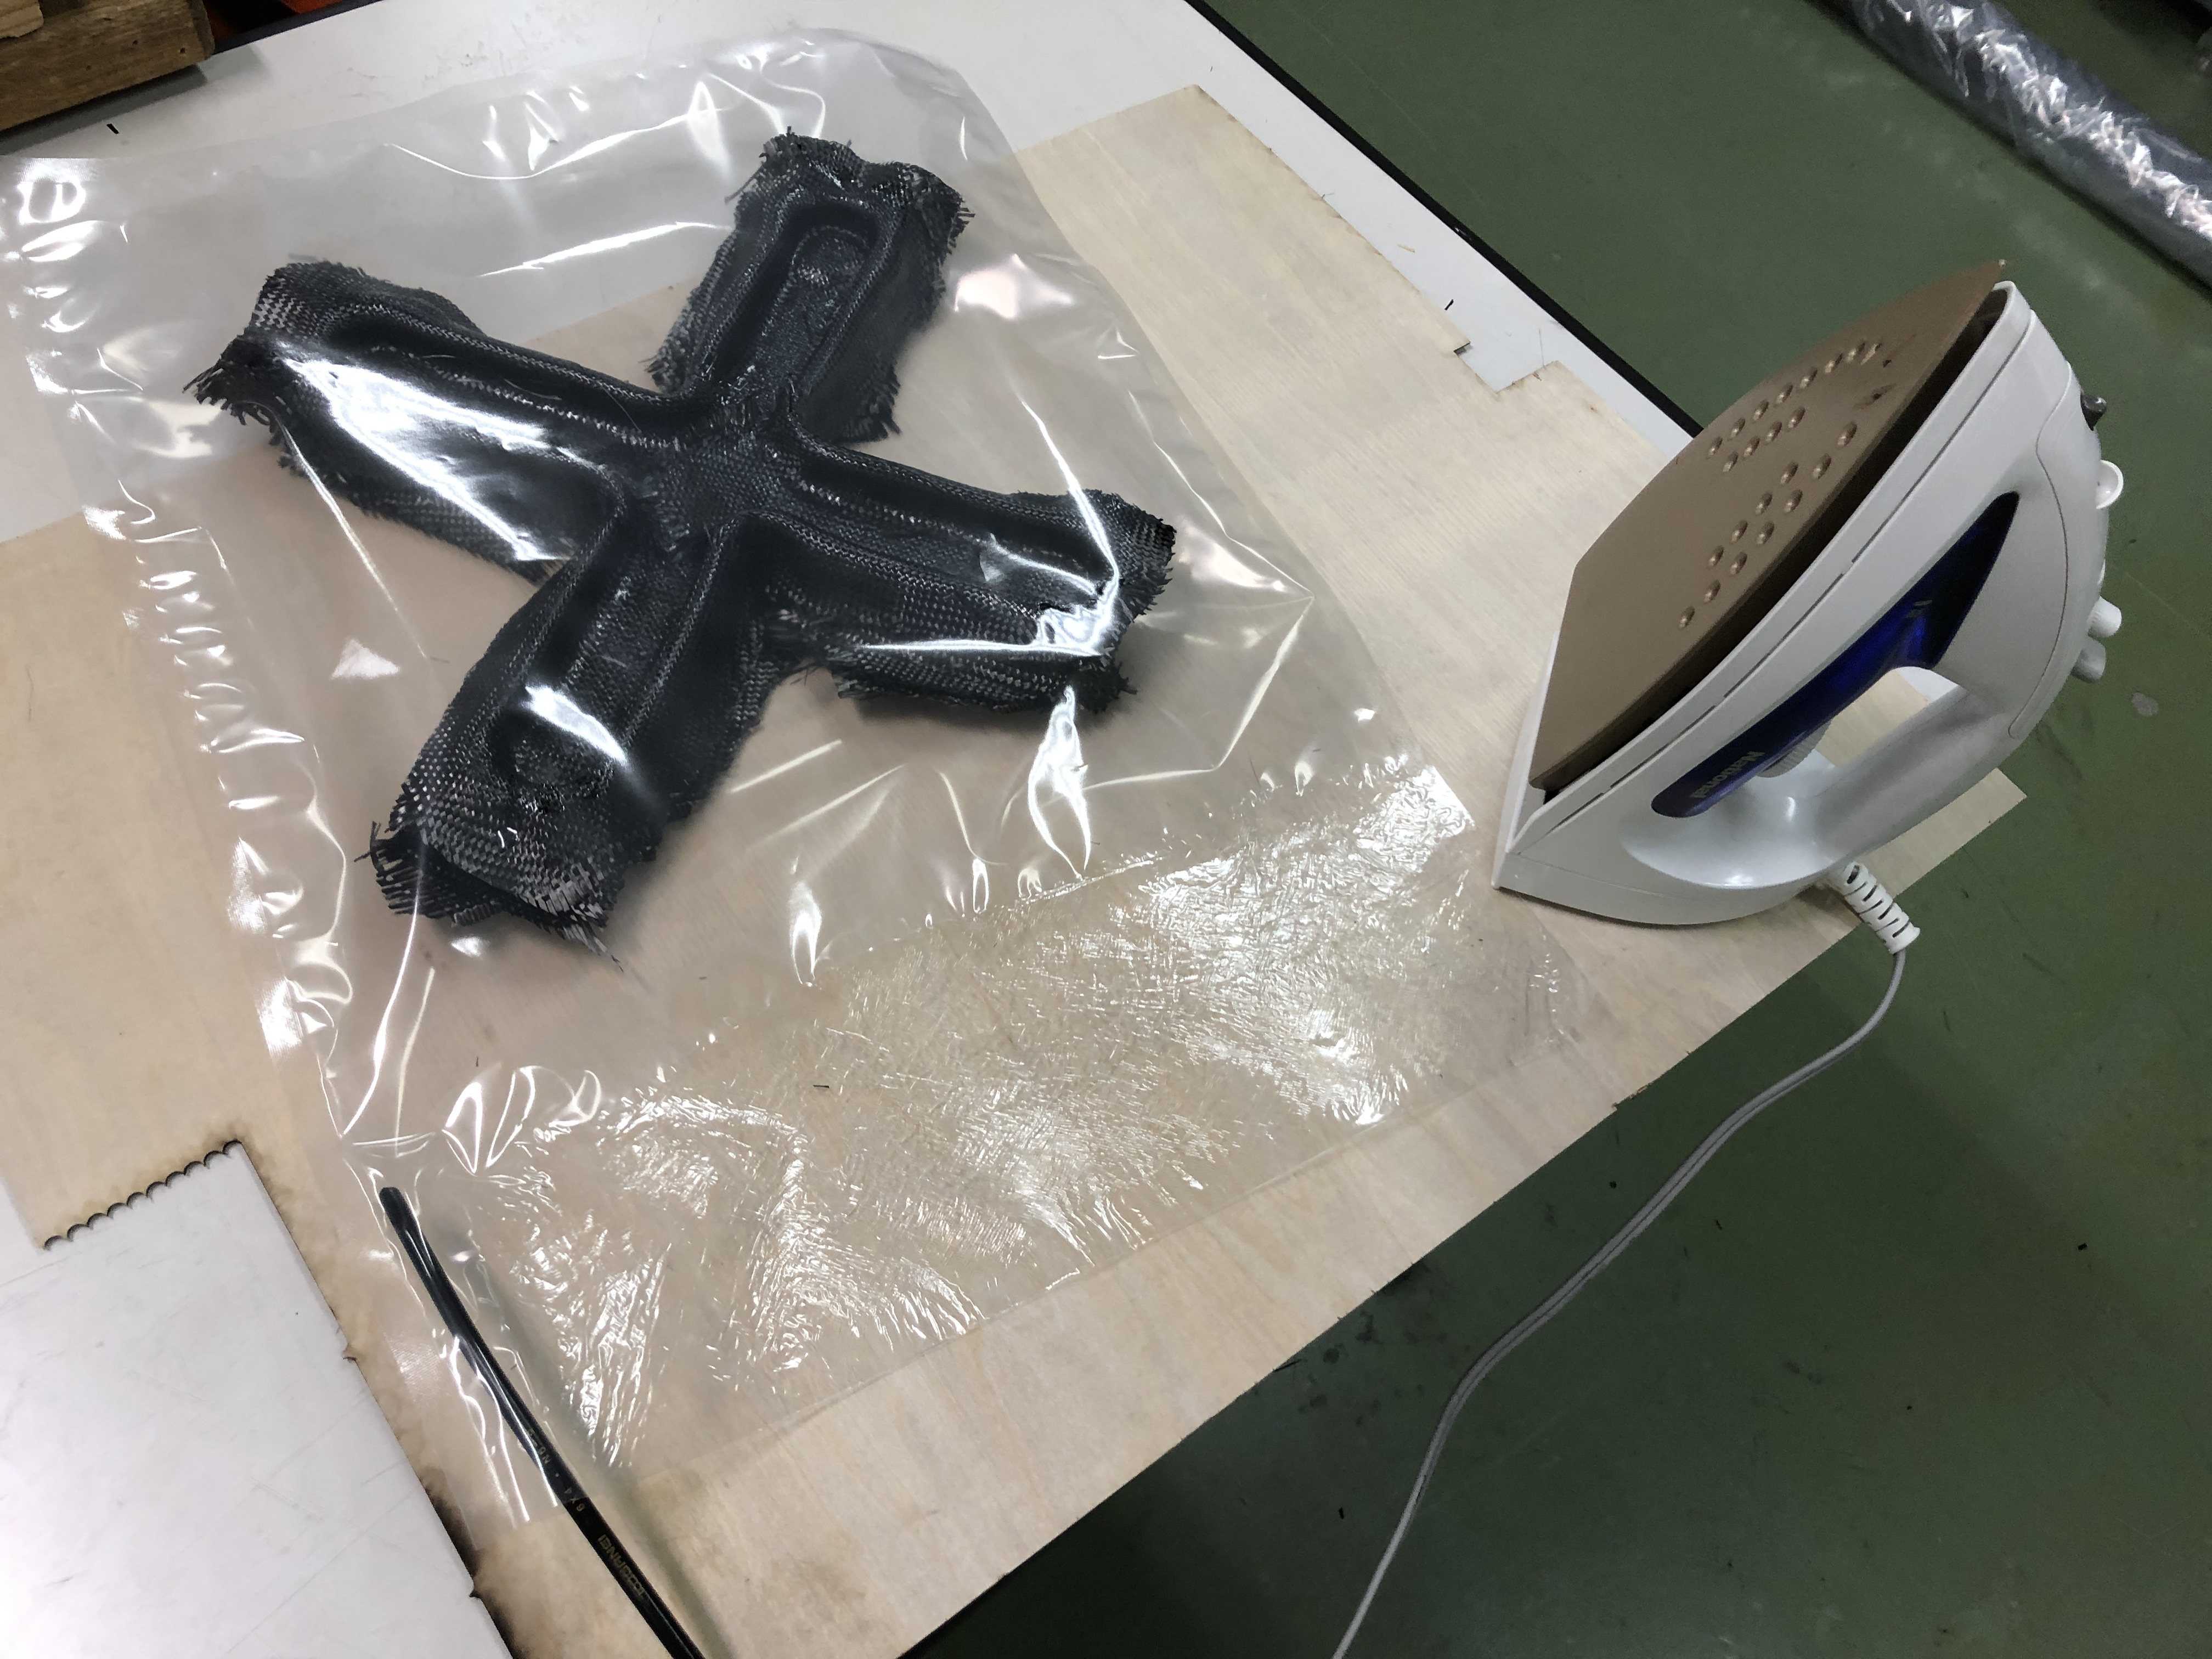
\includegraphics[width=120mm]{img/13.JPG}
    \end{center}
  \caption{真空引き前のフレーム}
 \label{fig:robot}
\end{figure}

\begin{figure}[htbp]
  \begin{center}
    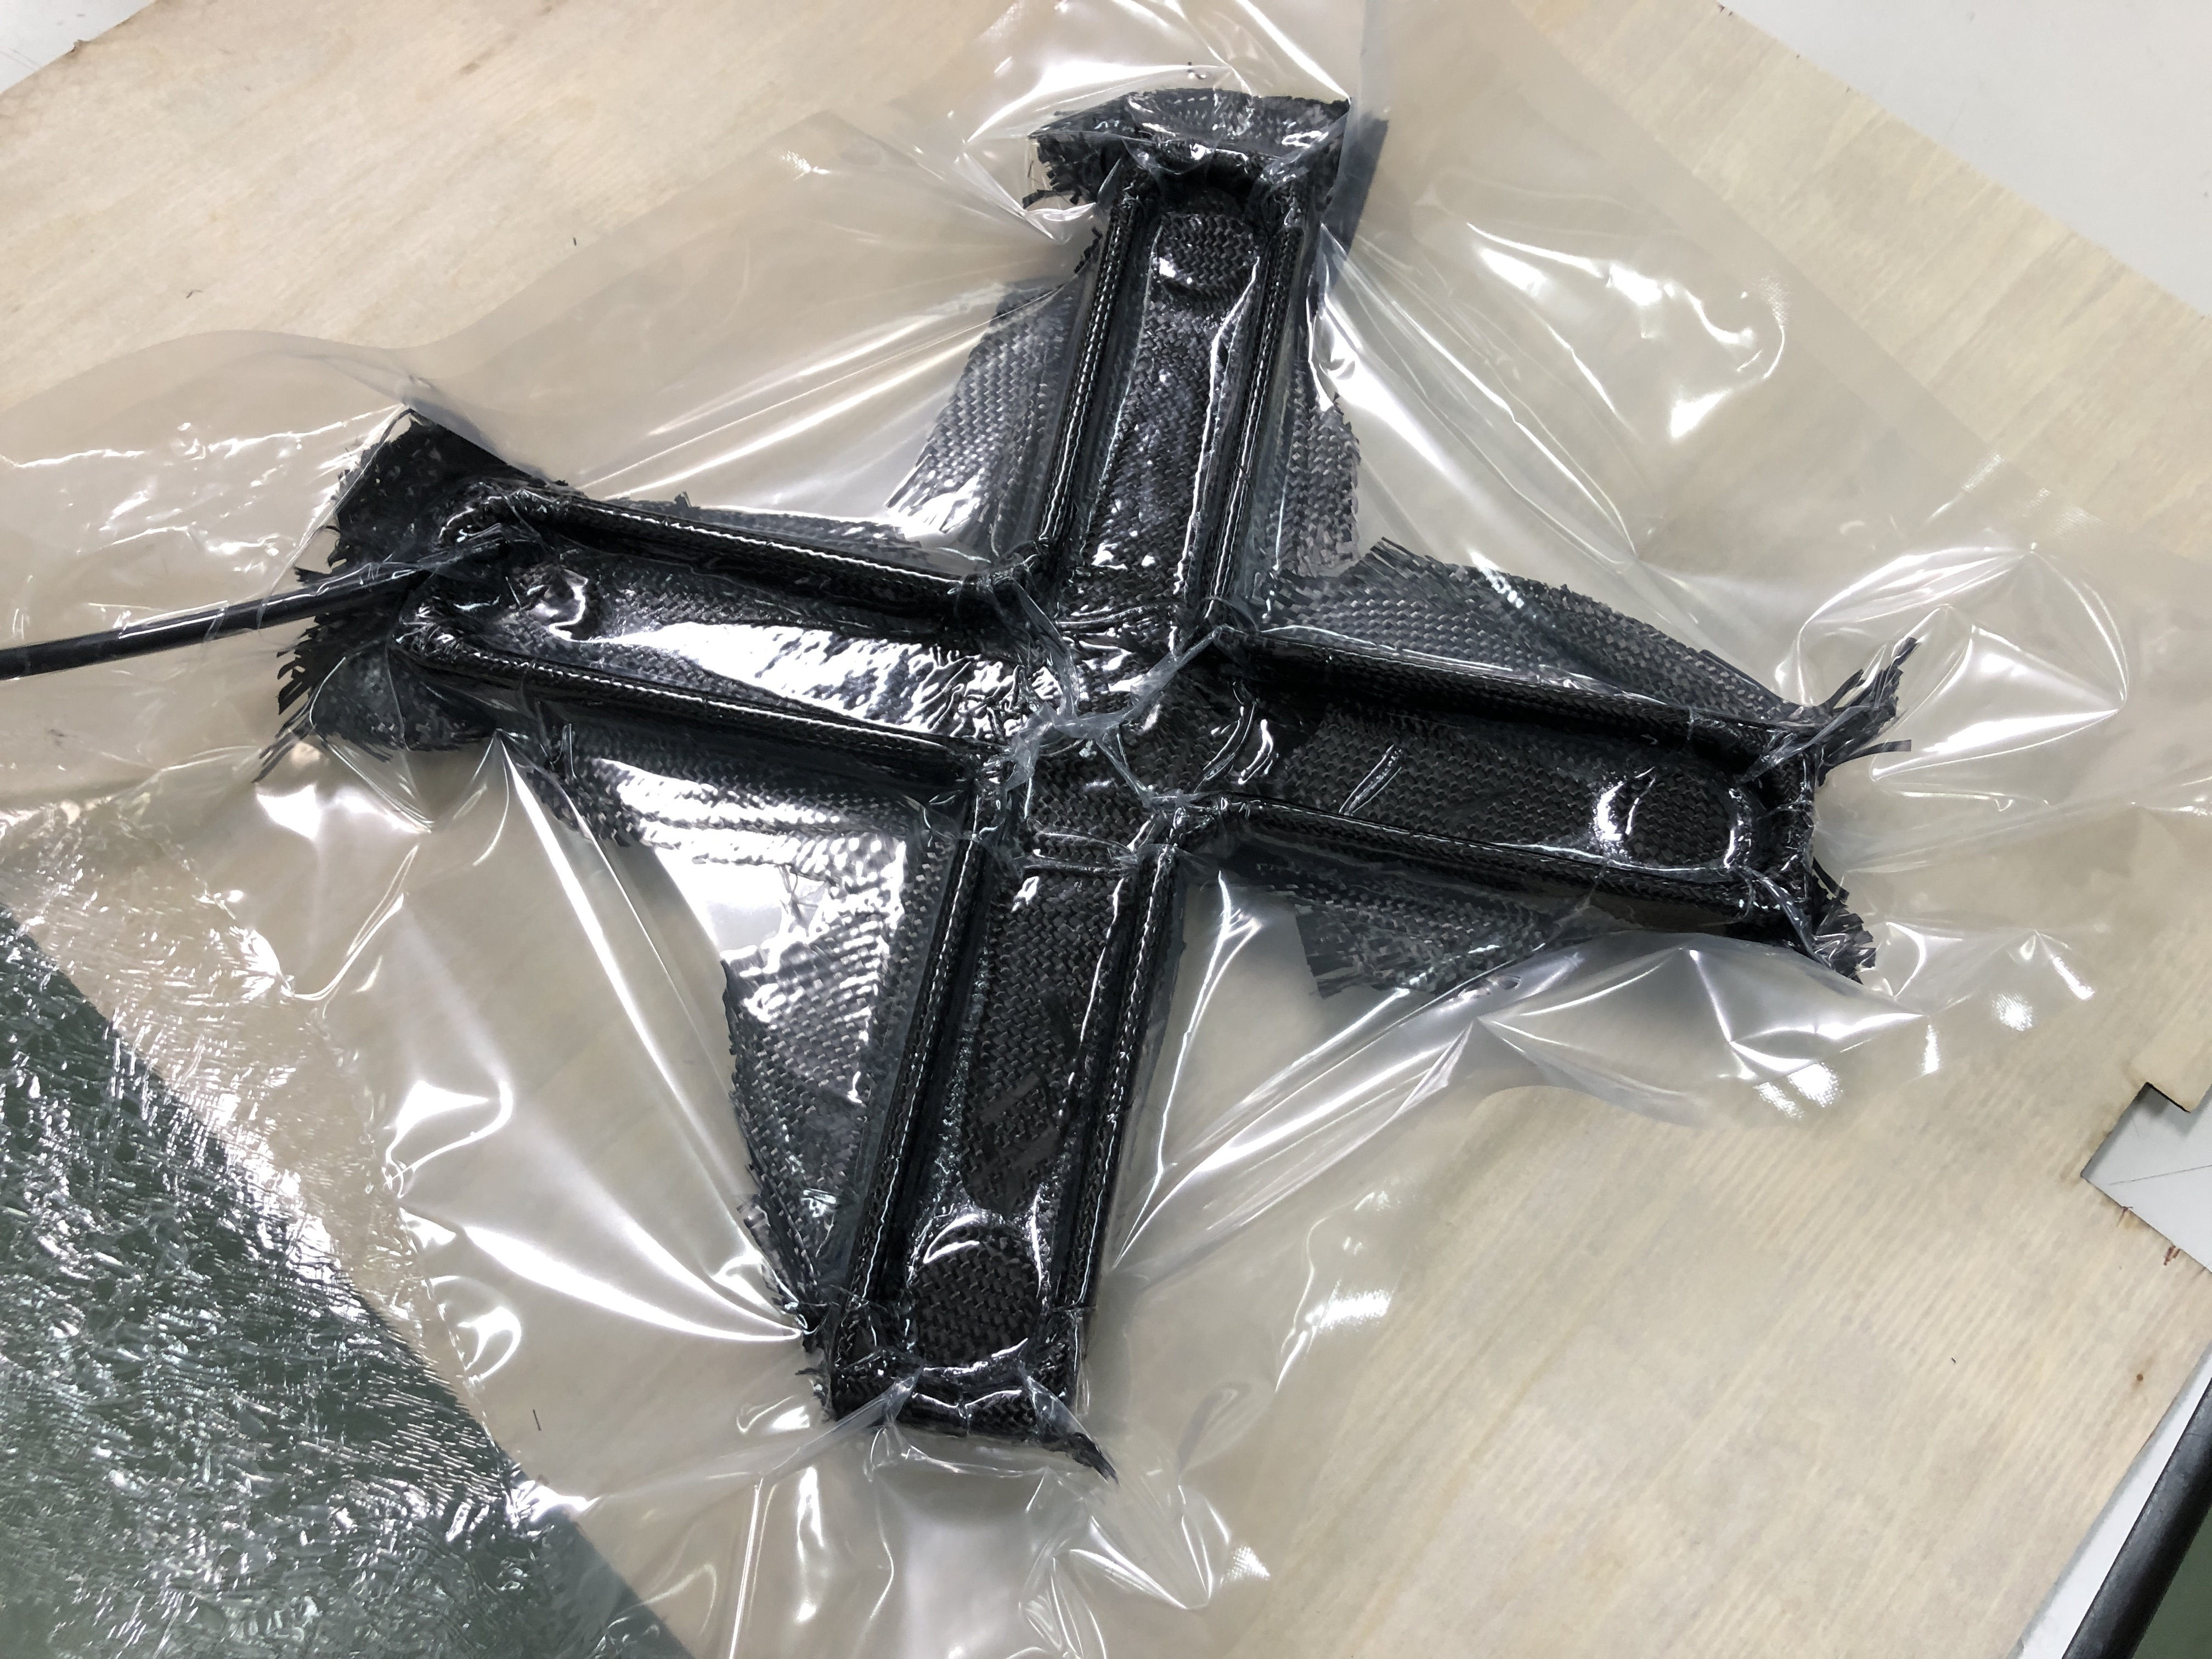
\includegraphics[width=120mm]{img/14.JPG}
    \end{center}
  \caption{真空引き後アイロンで密閉されたフレーム}
 \label{fig:robot}
\end{figure}

\section{バリ取り,ヤスリ掛け}
24時間以上が経過し完全移行化したフレームは,型から取り外しバリを糸ノコで切り落とし,やすり掛けを行い完成となる.

\begin{figure}[htbp]
  \begin{center}
    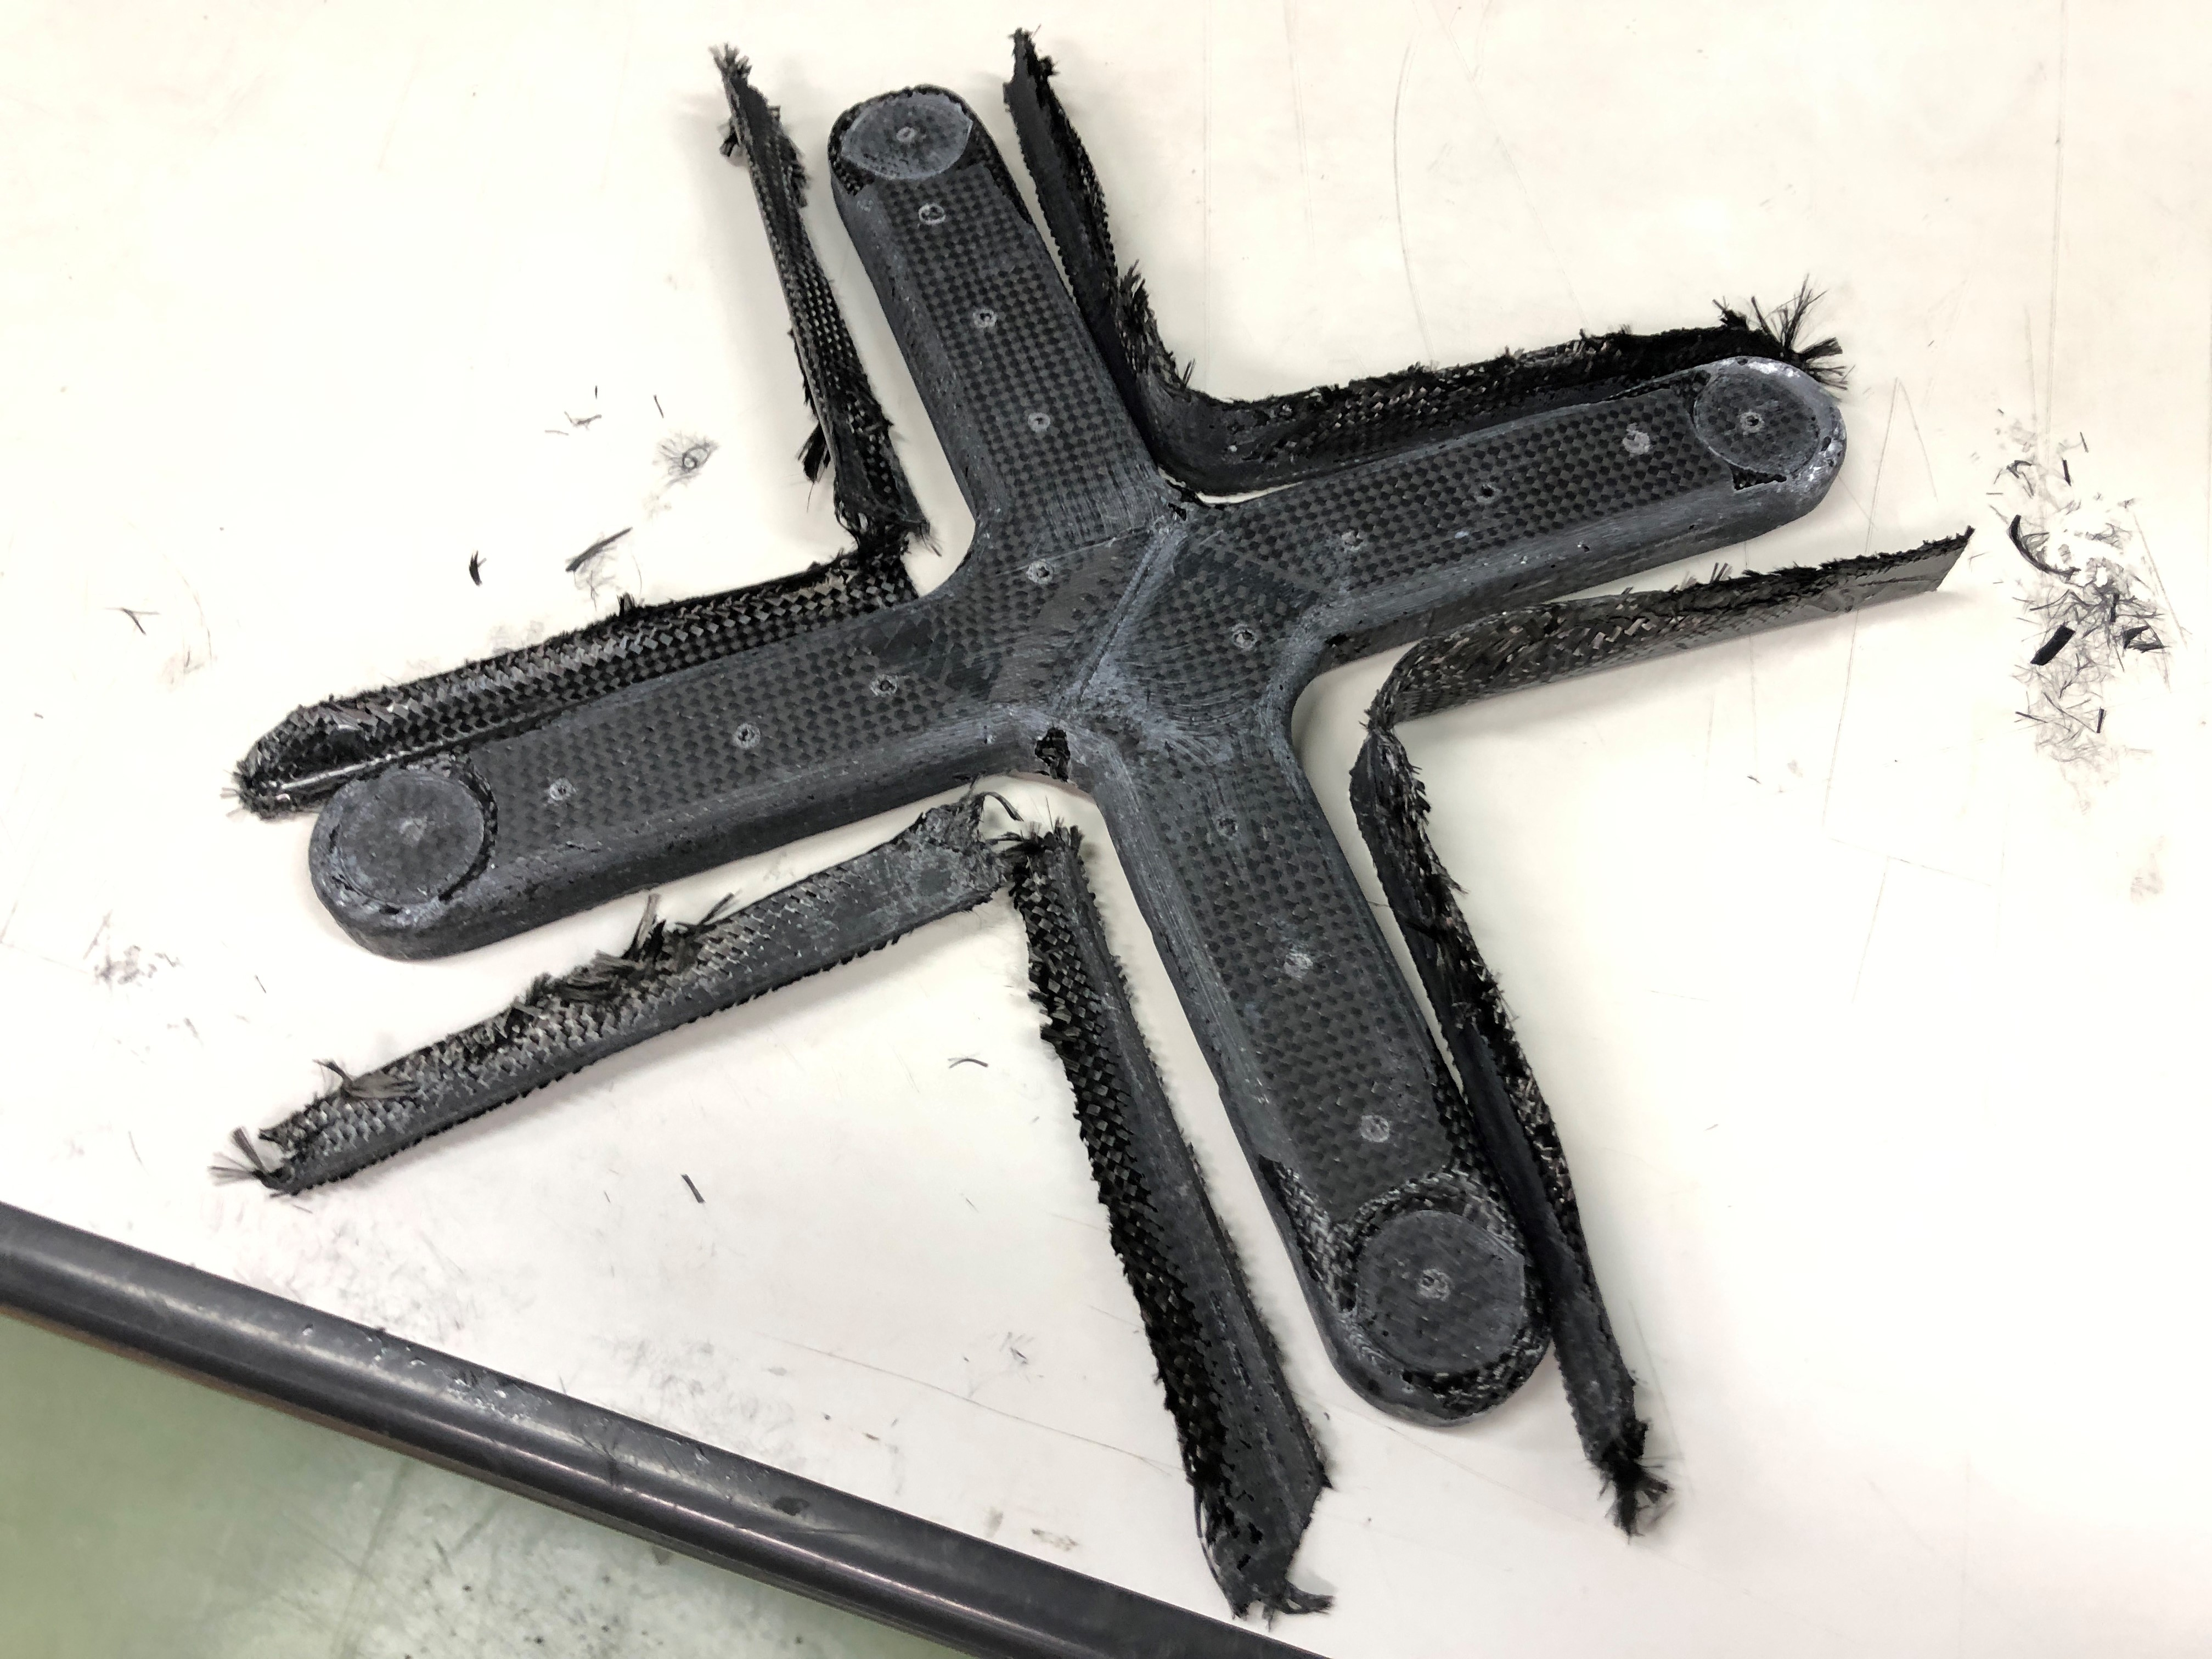
\includegraphics[width=120mm]{img/15.JPG}
    \end{center}
  \caption{バリ取り後のフレーム}
 \label{fig:robot}
\end{figure}

\begin{figure}[htbp]
  \begin{center}
    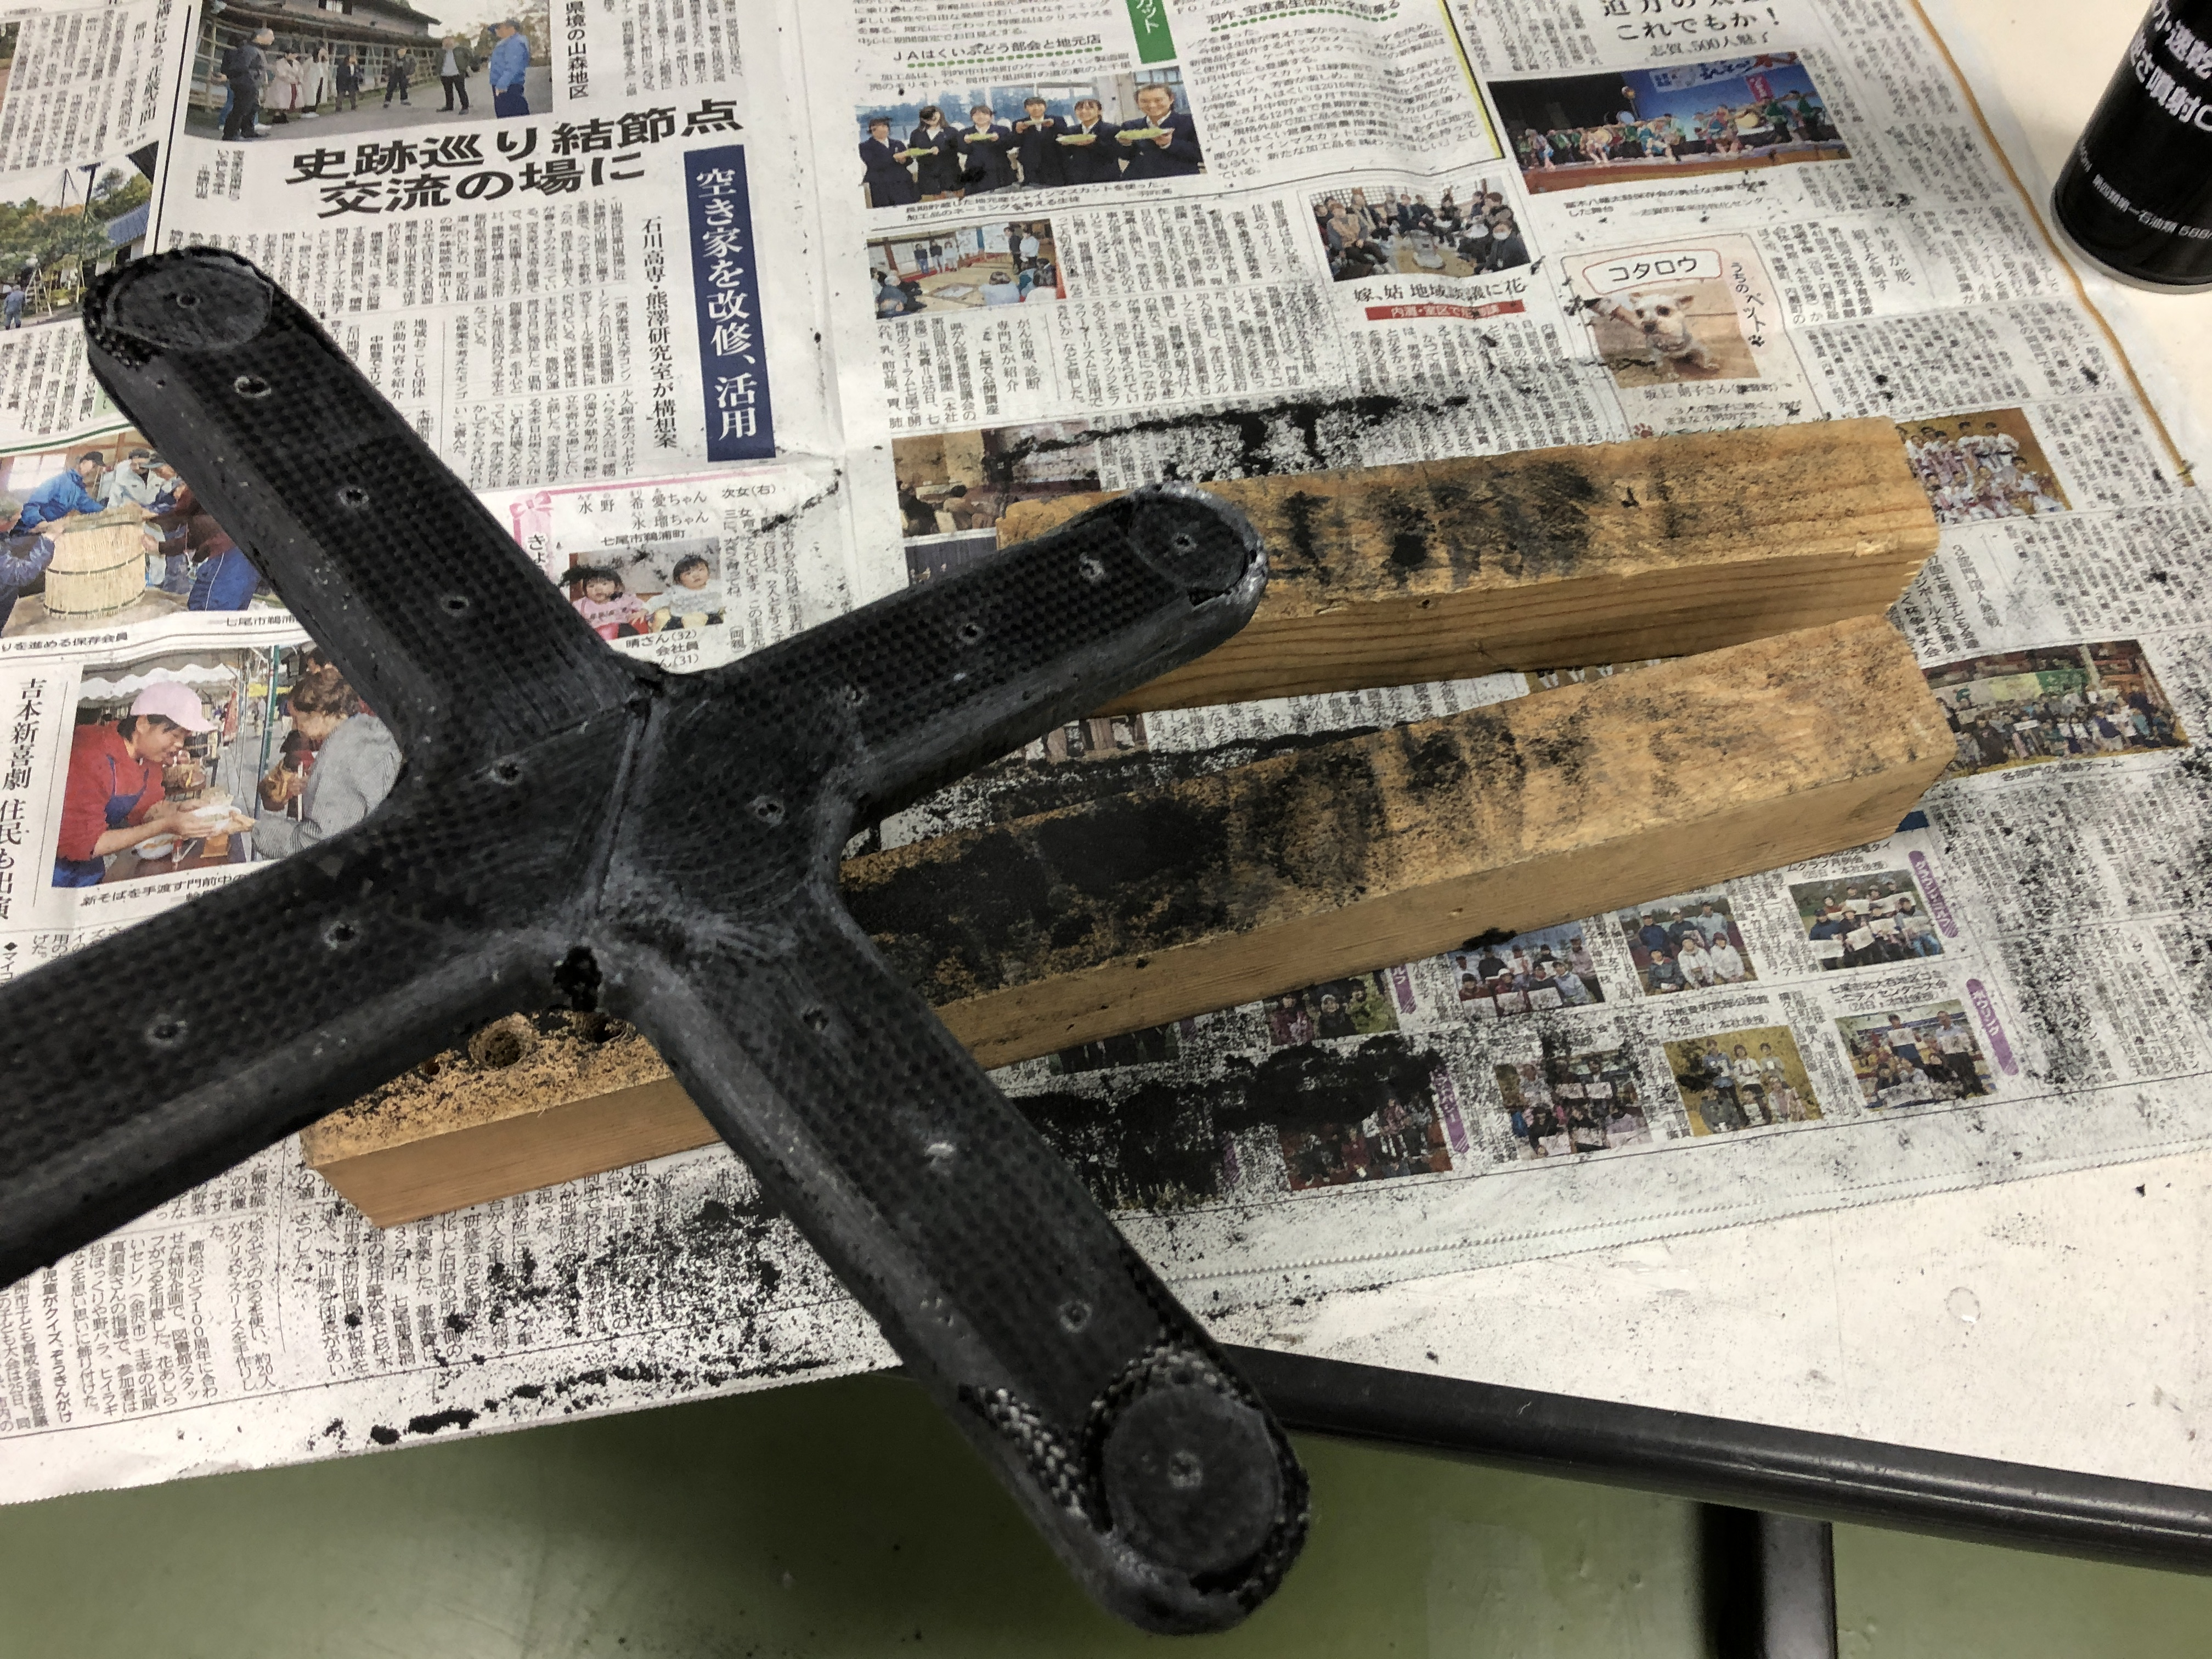
\includegraphics[width=120mm]{img/16.JPG}
    \end{center}
  \caption{ヤスリをかけ仕上げられたフレーム}
 \label{fig:robot}
\end{figure}

\section{立体フレーム製作過程においてのまとめ}
\subsection{離型剤について}
立体フレーム製作において積層硬化後,離型に車用ワックスとエポキシ樹脂用スプレー型離型剤を用いた,ワックスは代用品ではあるが樹脂と型との間に膜の役割として塗ることができるため比較的容易に離型することができる.ポリプロピレン製のフィルムは,立体の複雑な形に対しての柔軟性がなかったため使用をしなかった,また,ワックスを用いての離型後も表面状態が異なった.
平面積層時同様にスプレー型の専用のものを使った場合,表面はつやがないマットな仕上がりとなった,しかし,散布する量にむらがあったり,量が多くなりすぎると表面に固着してしまい仕上がり面が綺麗にならなかった.
それに対しワックスを用いた場合は,仕上がりは艶のない面となった.
ワックスは固形であるため,手作業で量を調節しながら塗り込めるので,スプレー式より最適であった,

\subsection{樹脂吸着シートについて}
立体積層においては平面積層に比べ多量の硬化剤を用いる.よって積層後に雌型の底の部分に樹脂の溜まりができてしまう.そのため余分な樹脂を除去するために専用に吸着シートを用いた.しかし積層時にしわになってしまうとカーボンクロスに巻き込まれてしまい綺麗な積層が行えなかったため使用はしなかった.樹脂がたまる対策として,雌型に穴をあけて溜まらないように加工を施した.

\begin{figure}[htbp]
  \begin{center}
    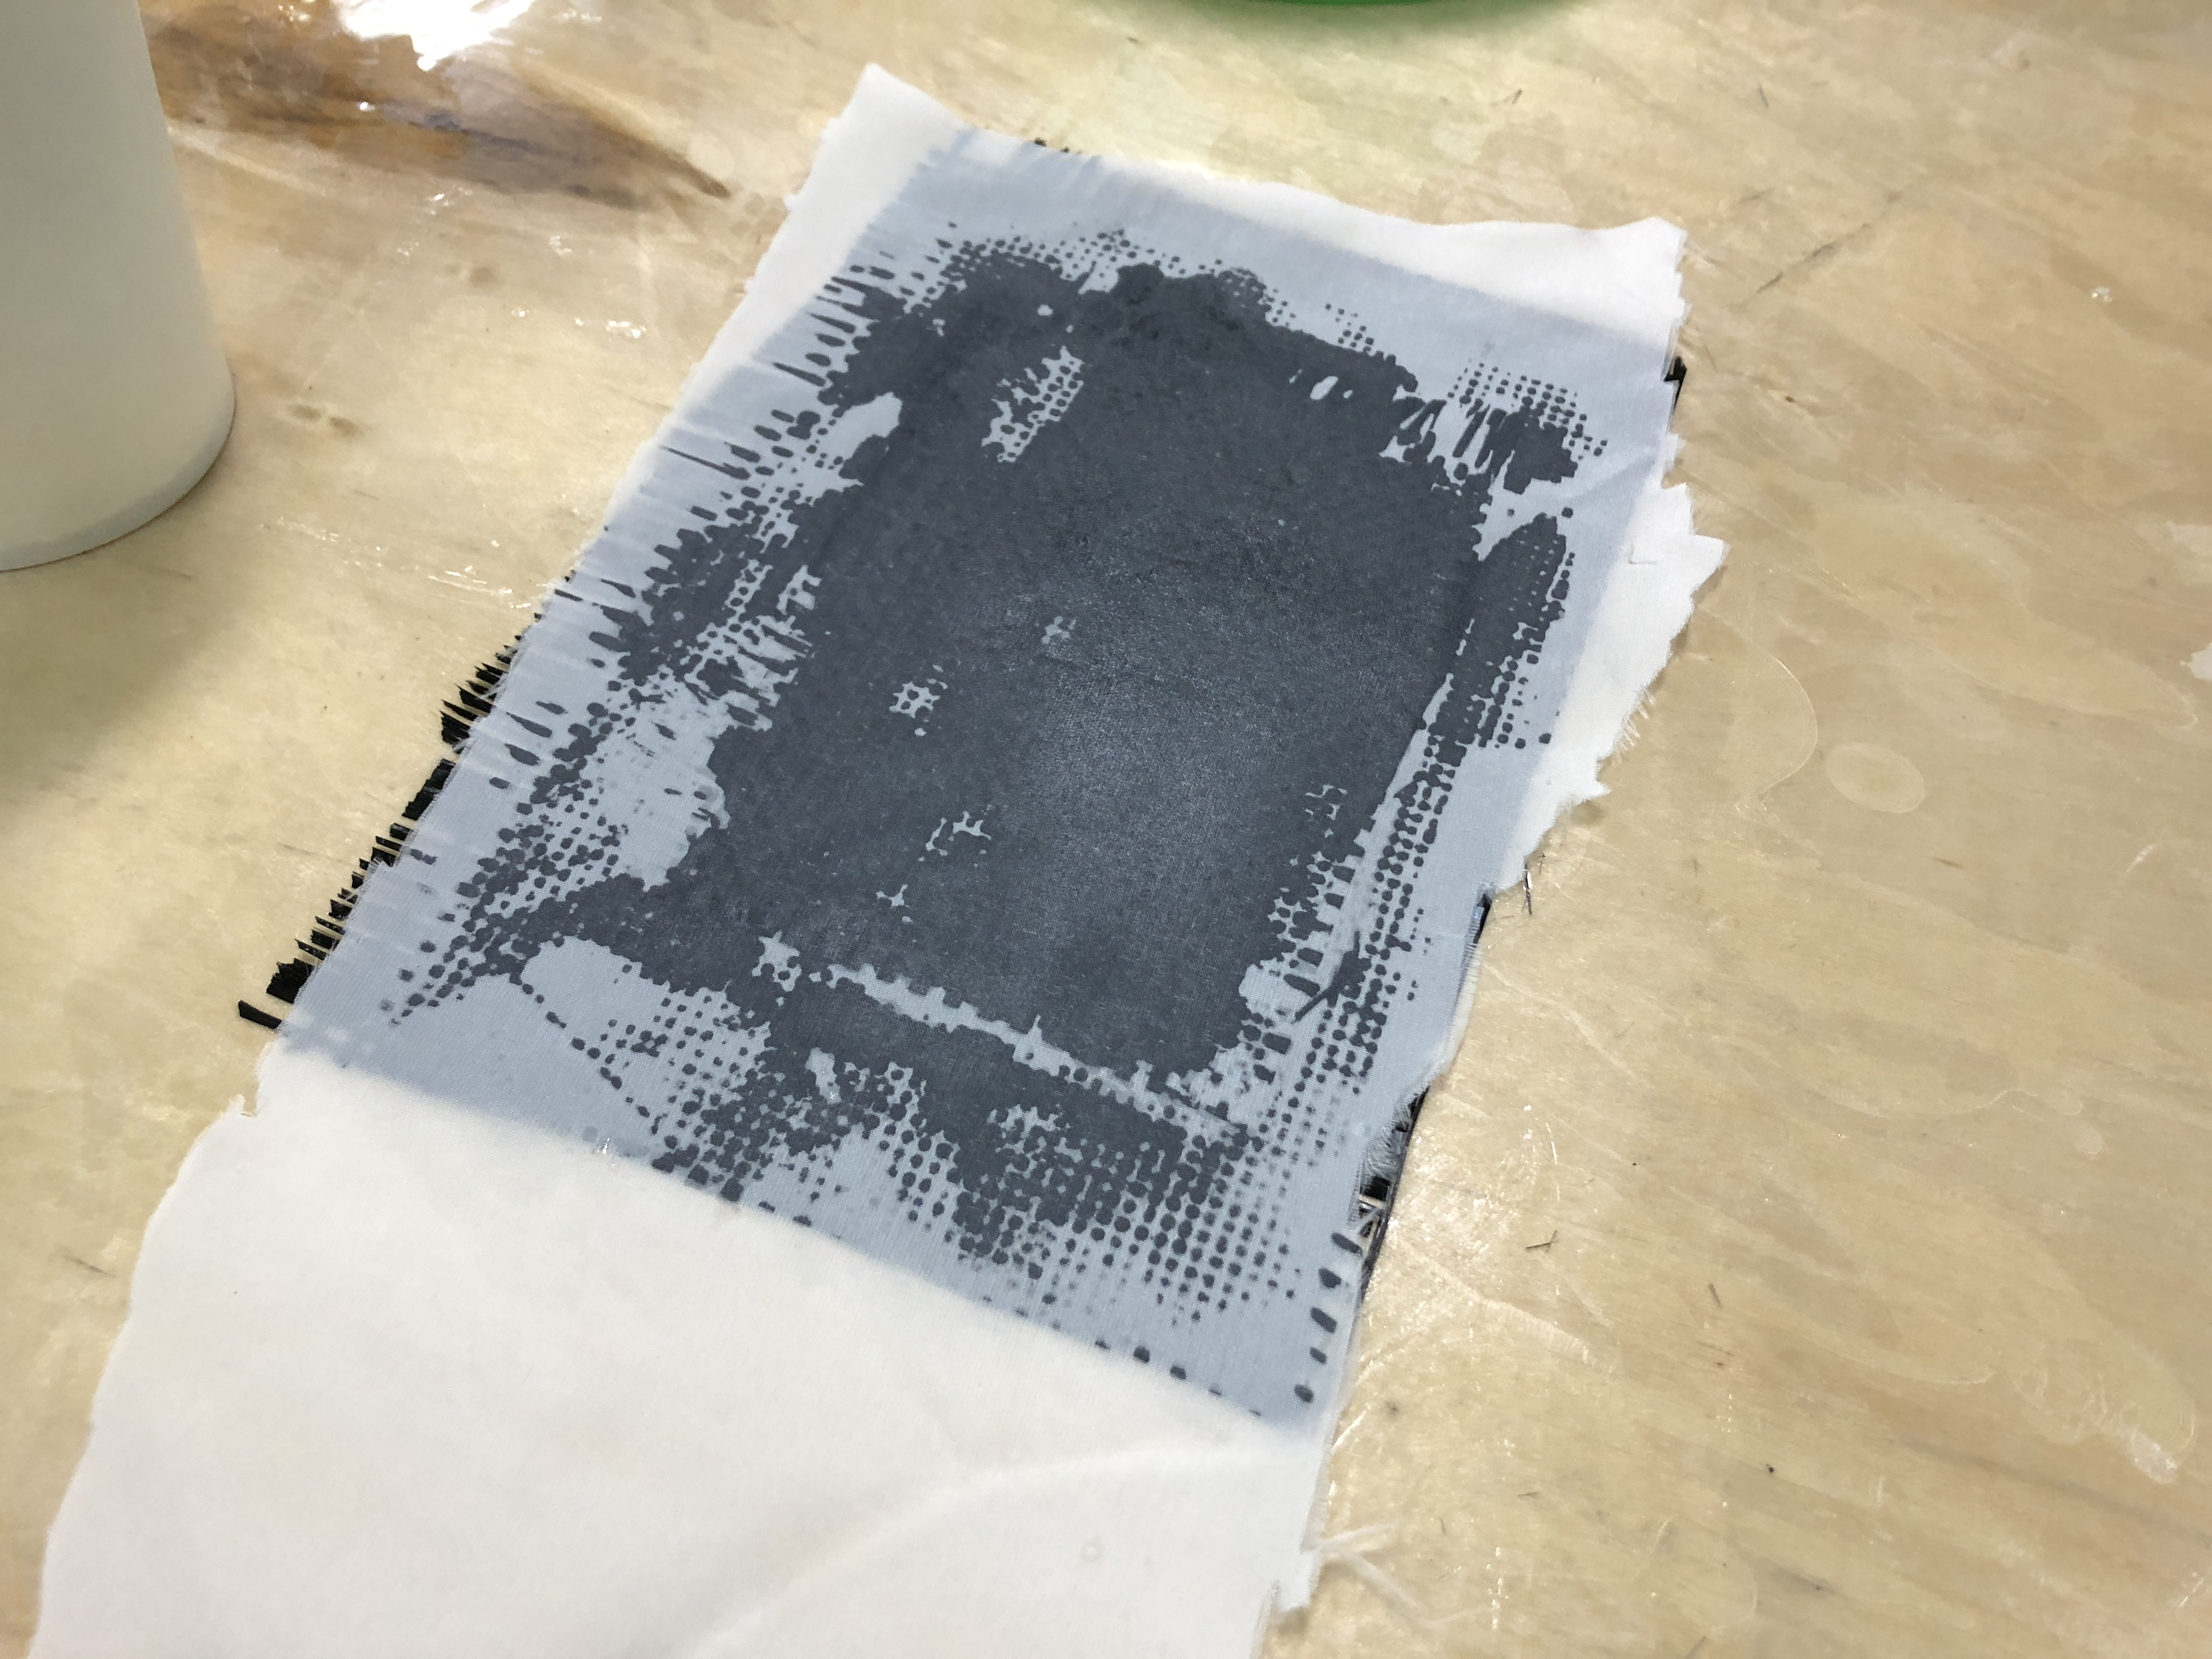
\includegraphics[width=120mm]{img/25.JPG}
    \end{center}
  \caption{樹脂吸着シート}
 \label{fig:robot}
\end{figure}

\begin{figure}[htbp]
  \begin{center}
    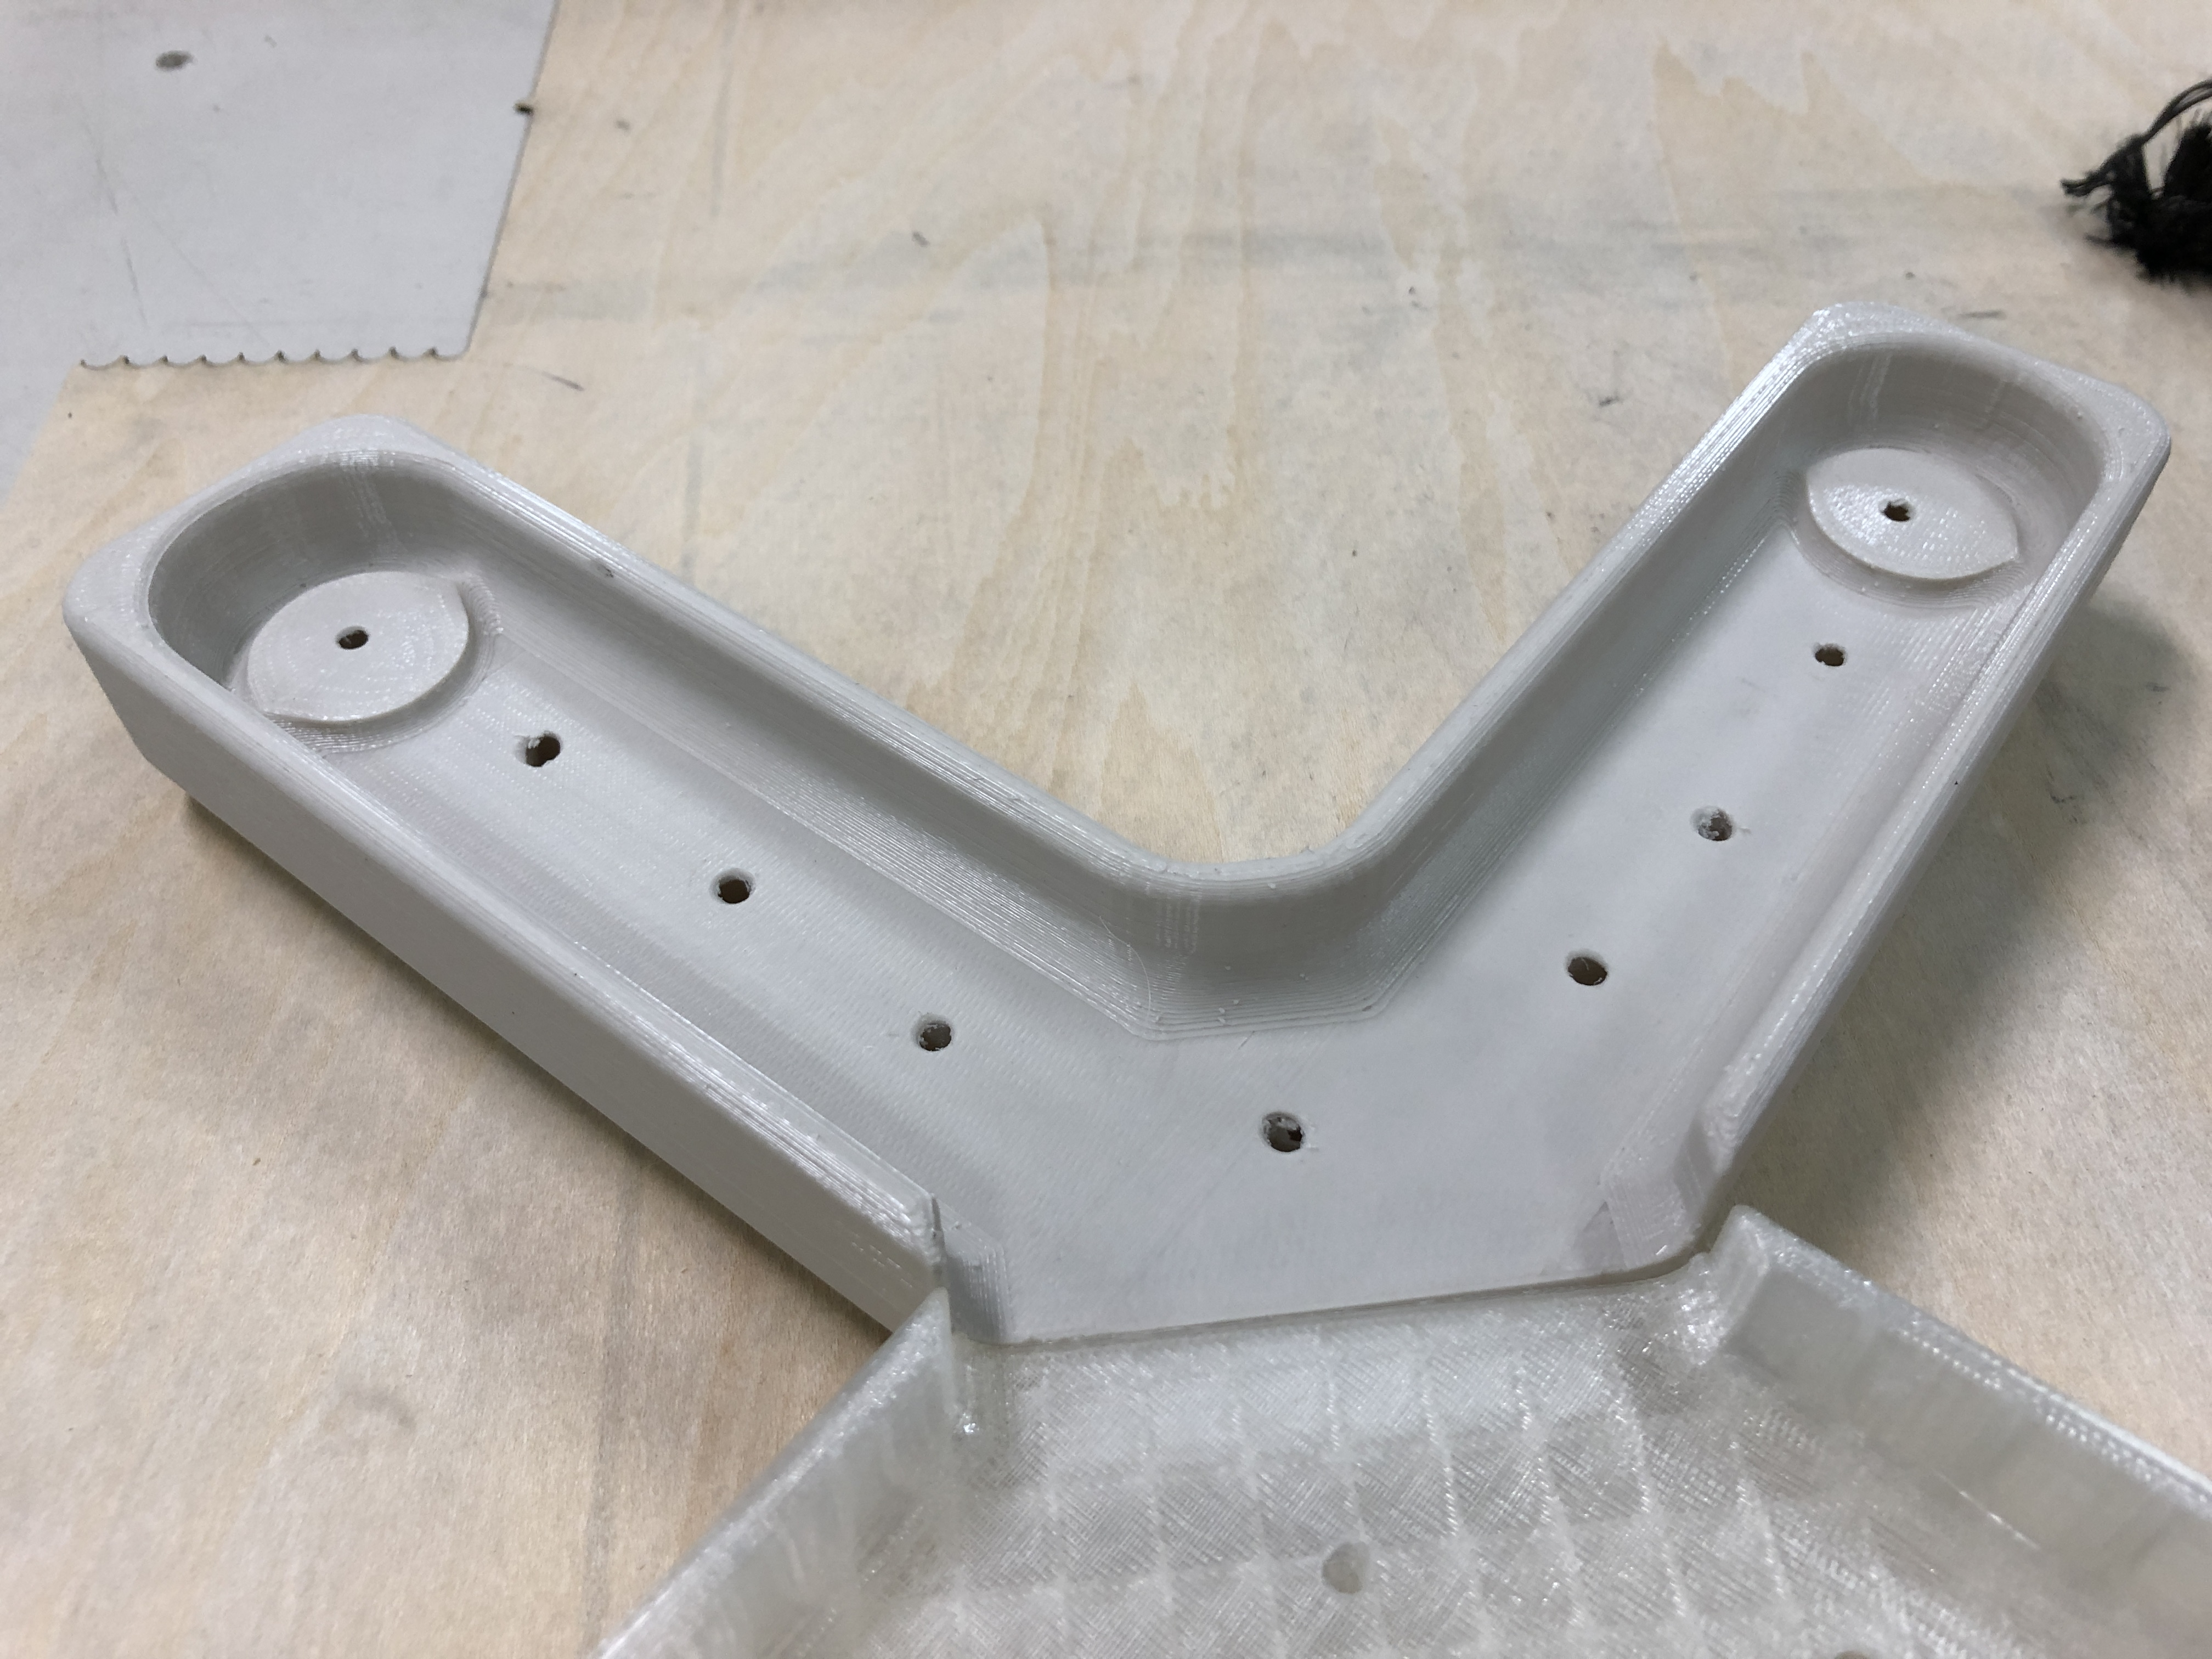
\includegraphics[width=120mm]{img/26.JPG}
    \end{center}
  \caption{穴あけ加工された雌型}
 \label{fig:robot}
\end{figure}

\subsection{雄型,雌型を用いての成型について}
真空引きで成型を行う以前に,雄型と雌型を用いての成型方法を試みた.雌型にカーボンシート,樹脂吸着シートを積層し,雄型をはめ合わせおもりをのせて成型する.しかし,雄型と雌型のはめ合いが相枚数次第で変わってしまう.そのためはめ合わせがきつくなりすぎると,硬化後の離型がとても困難だったため真空引きが立体積層において適している.

\begin{figure}[htbp]
  \begin{center}
    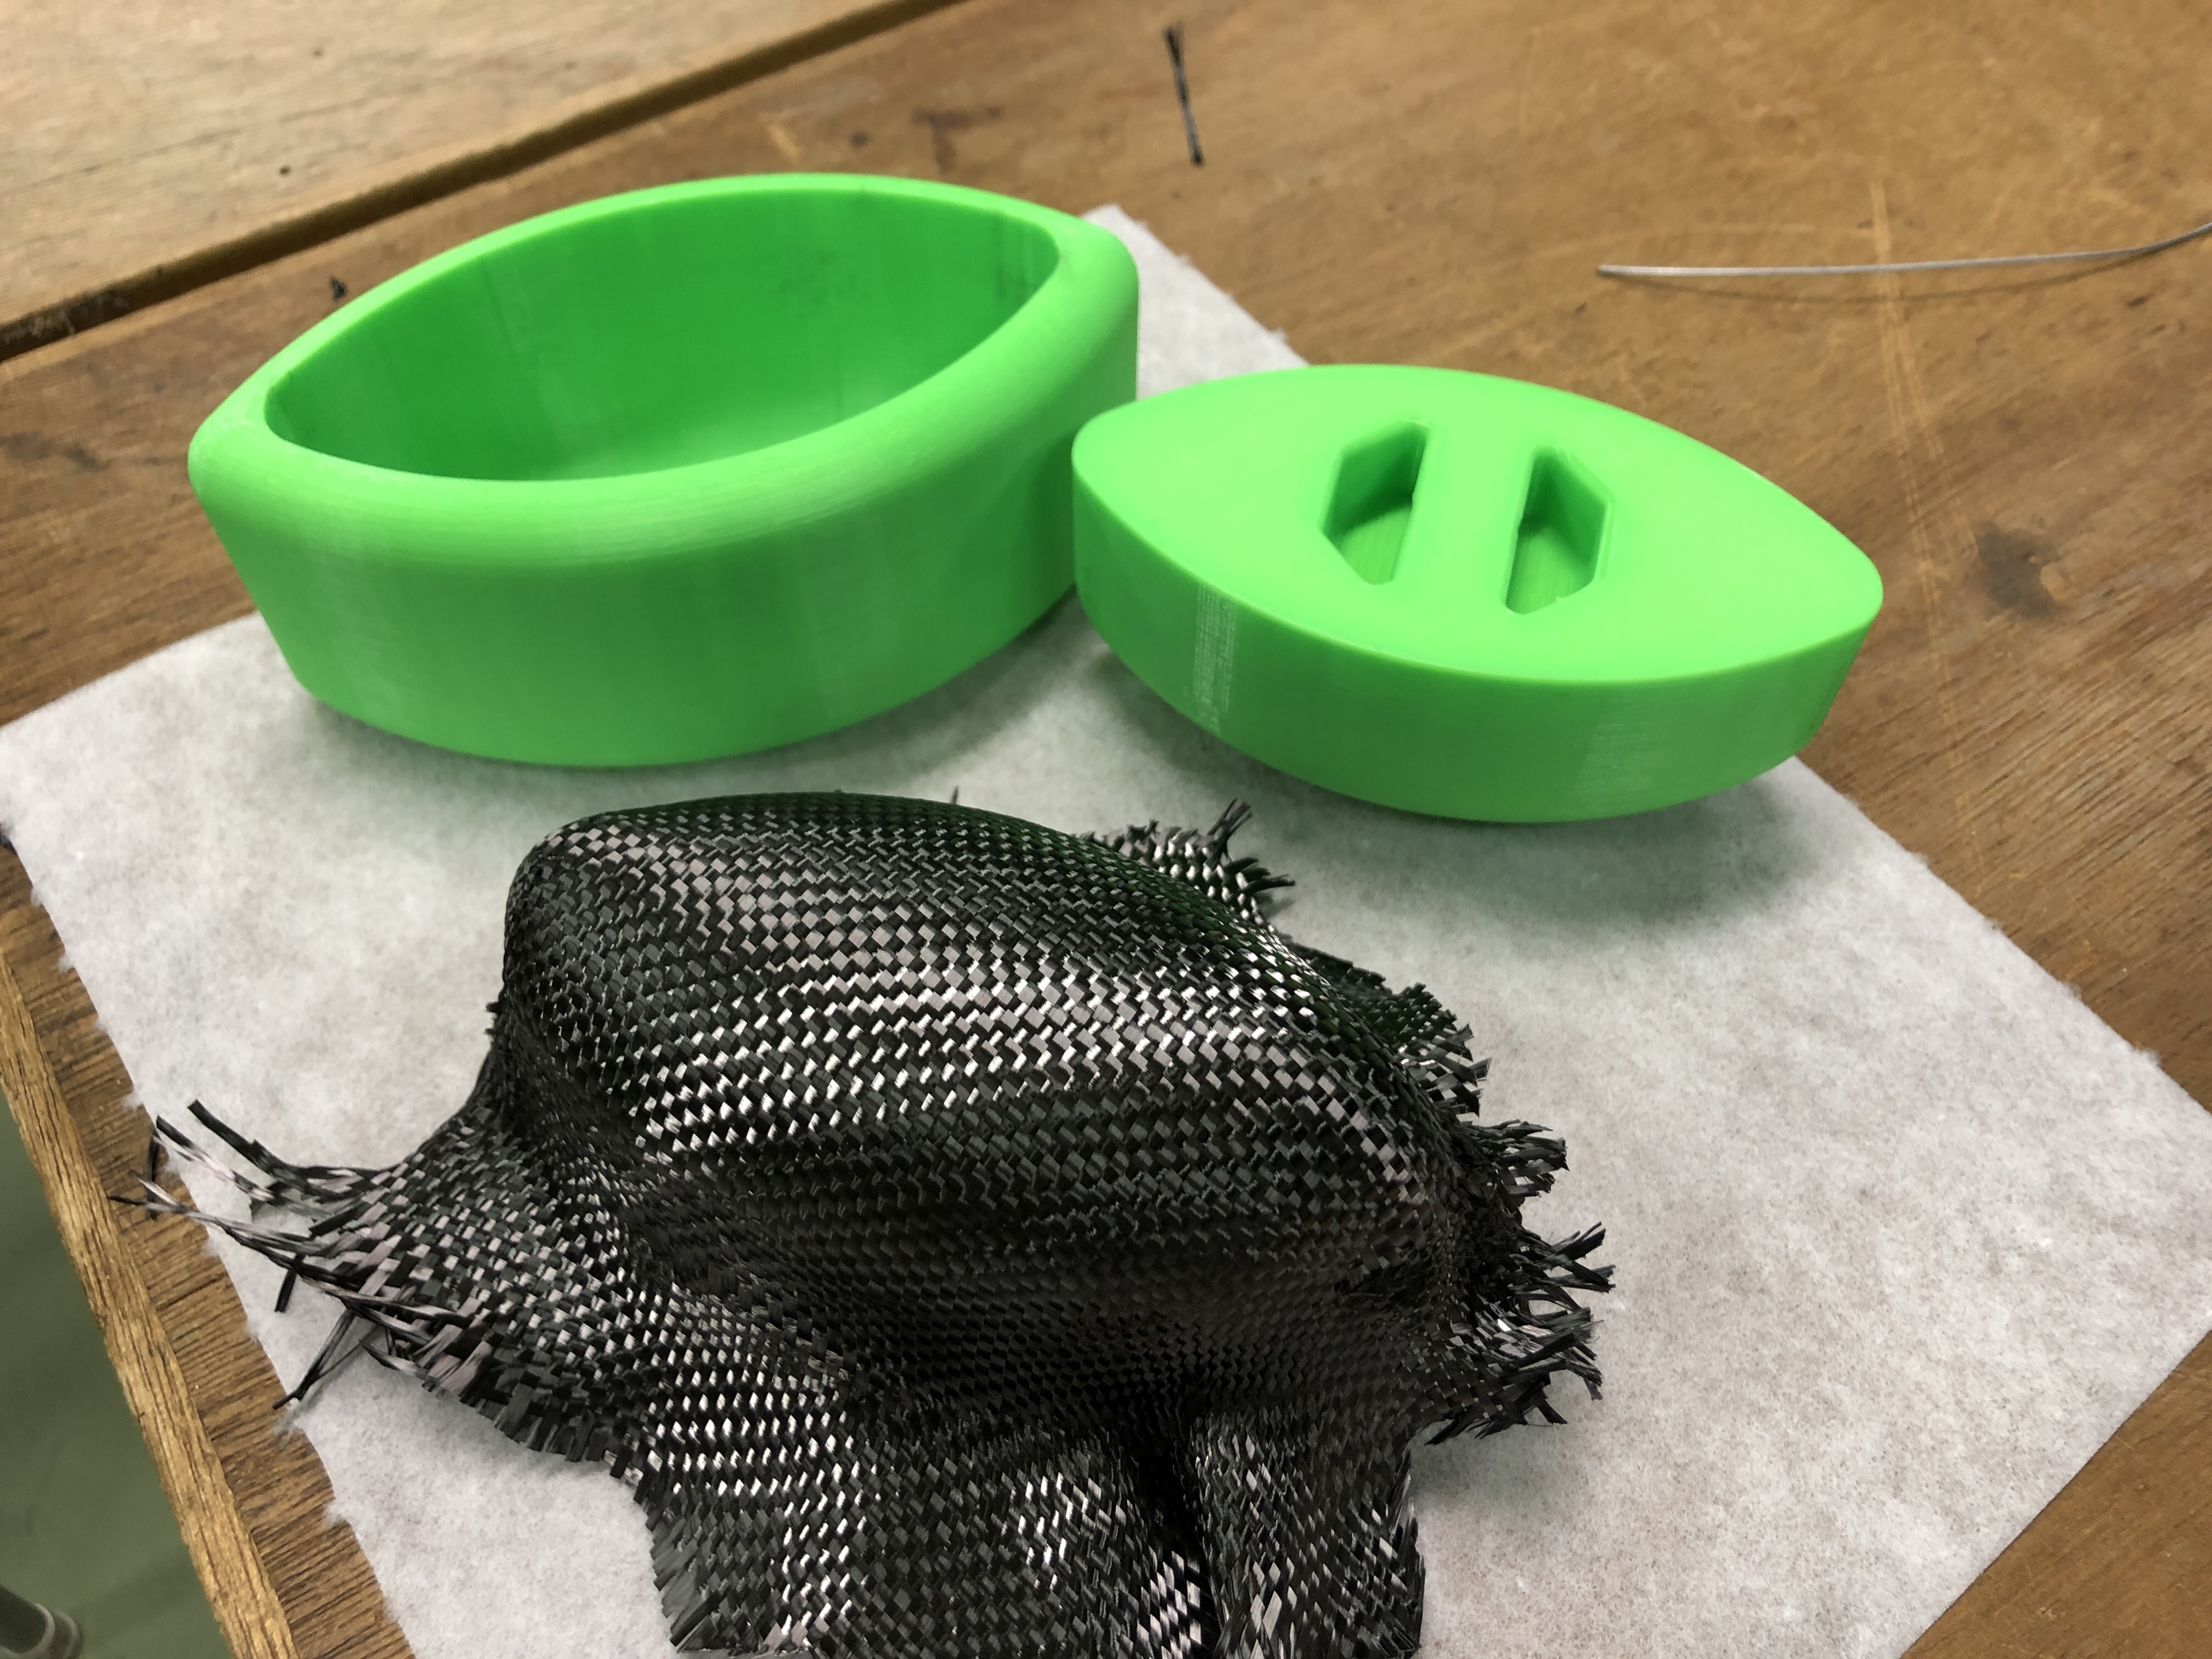
\includegraphics[width=120mm]{img/27.JPG}
    \end{center}
  \caption{雄型と雌型}
 \label{fig:robot}
\end{figure}

\begin{figure}[htbp]
  \begin{center}
    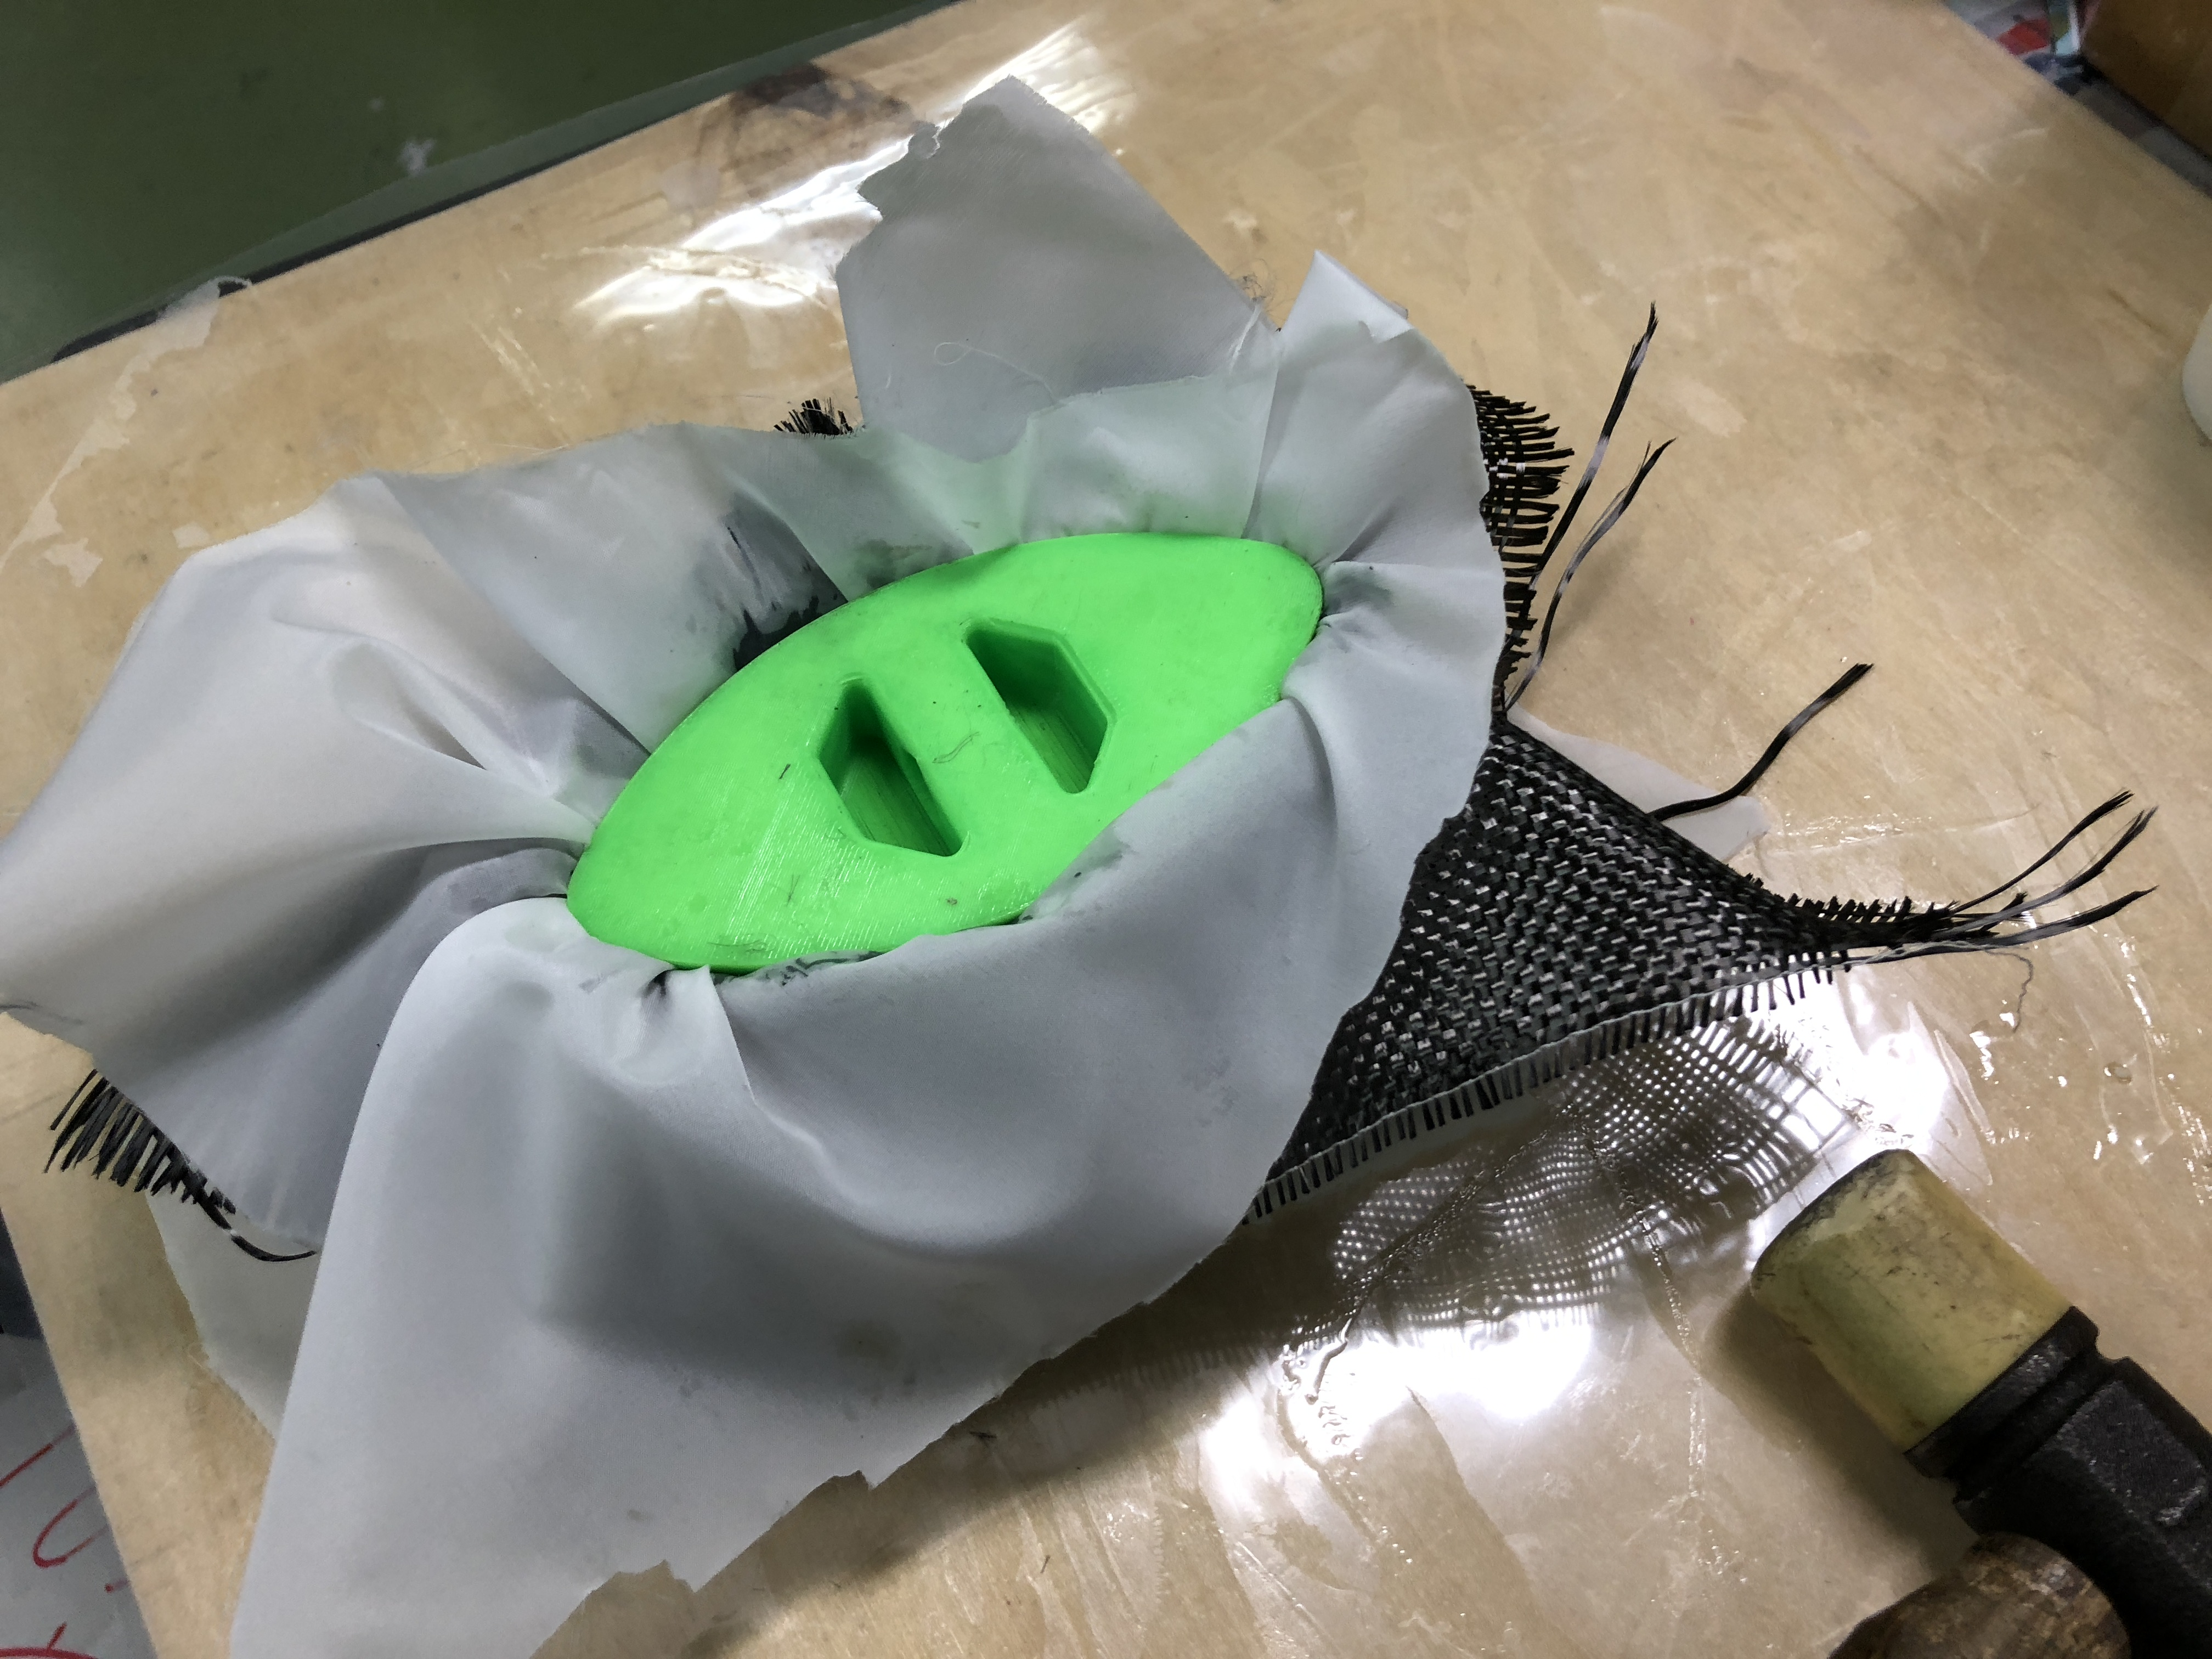
\includegraphics[width=120mm]{img/28.JPG}
    \end{center}
  \caption{はめ合わせ後の型}
 \label{fig:robot}
\end{figure}




\chapter{強度曲げ試験}
簡易的ではあるが.平面フレームと立体フレームの強度曲げ試験を行った.

\section{試験方法}
試験方法としてアーム中央部の根元を固定し,モータ取り付け部の先端部分に,ペットボトル容器に水を入れた重さの違うおもりをつるし,たわみ量を計測した,5N以上かけた場合,は破損してしまう可能性がったため平面フレームは5Nまでの試験とした.立体フレームは引き続き行い,33Nまで順に荷重をかけた..

\begin{figure}[htbp]
  \begin{center}
    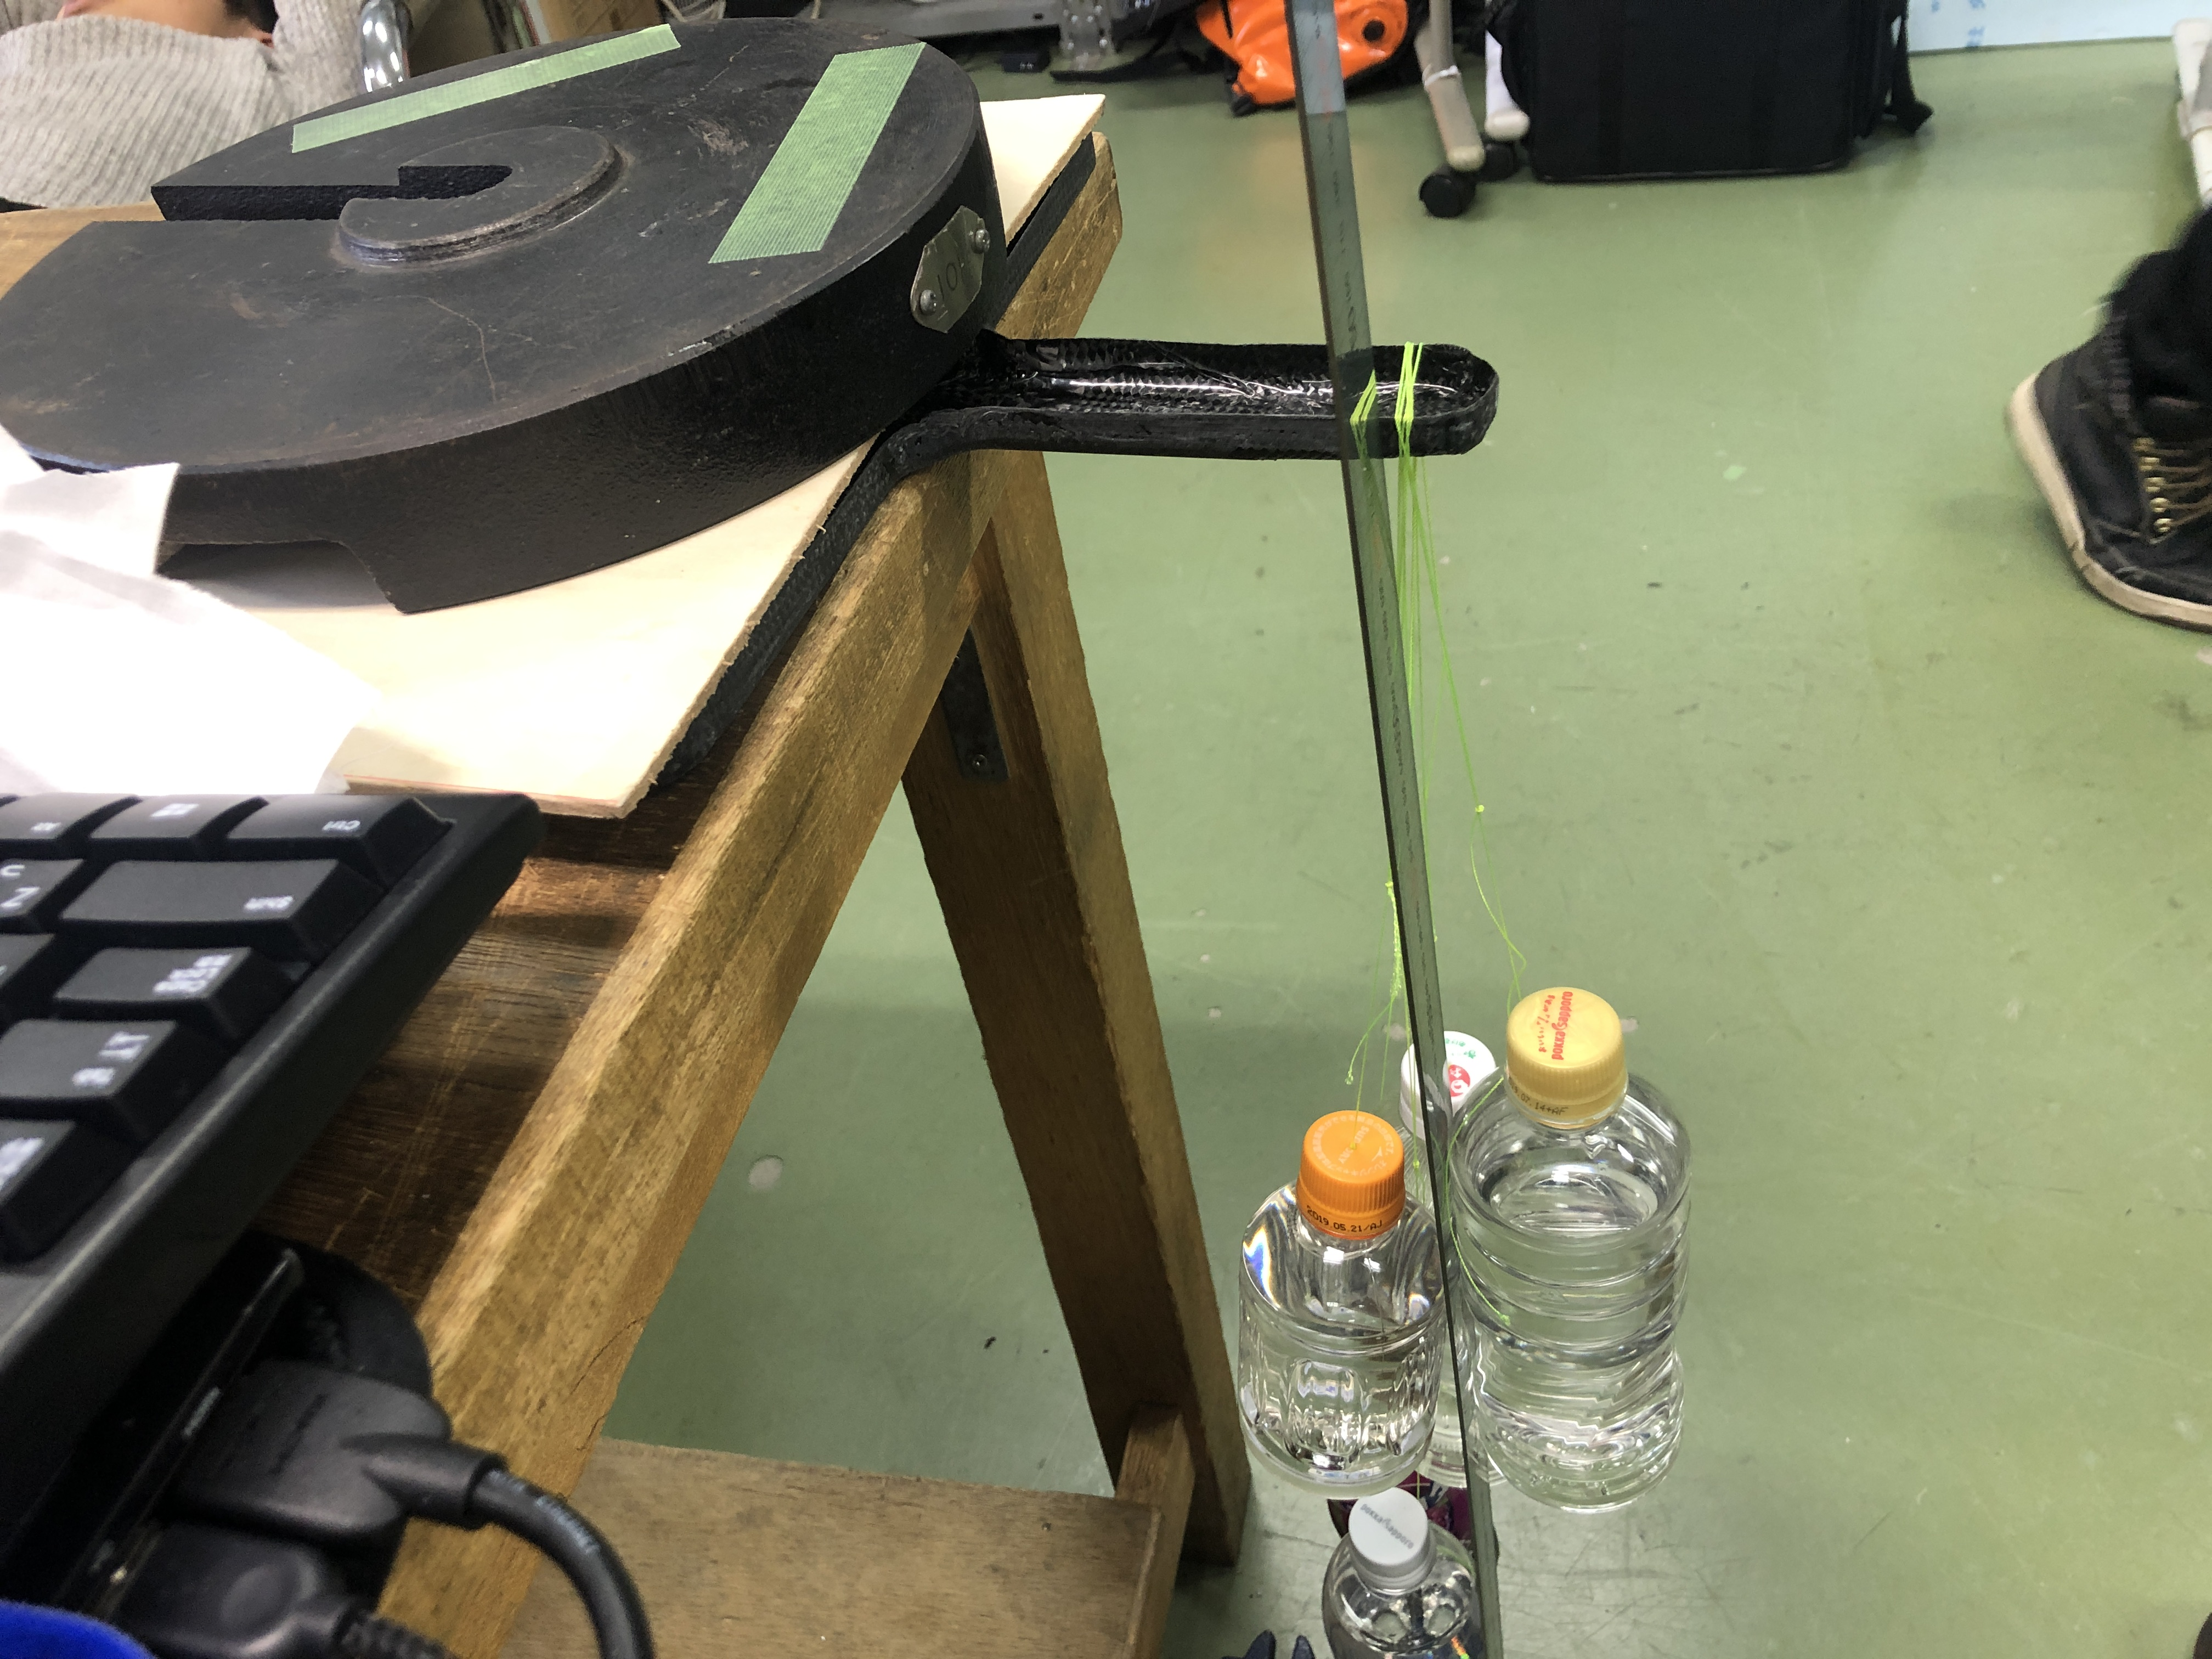
\includegraphics[width=120mm]{img/23.JPG}
    \end{center}
  \caption{おもりをつるした立体フレーム}
 \label{fig:robot}
\end{figure}

\section{試験結果}
図に示すグラフのように,平面フレームに比べ立体フレームの方が剛性が高いことがわかる.荷重が3N掛かった際に,たわみが9mmの平面フレームに対し,立体フレームは3mmである.また,5Nが掛かった際にはたわみが大幅に大きくなり平面フレームは24mm変形する.33Nの荷重がかかった立体フレームは13mm変形した.

\begin{figure}[htbp]
  \begin{center}
    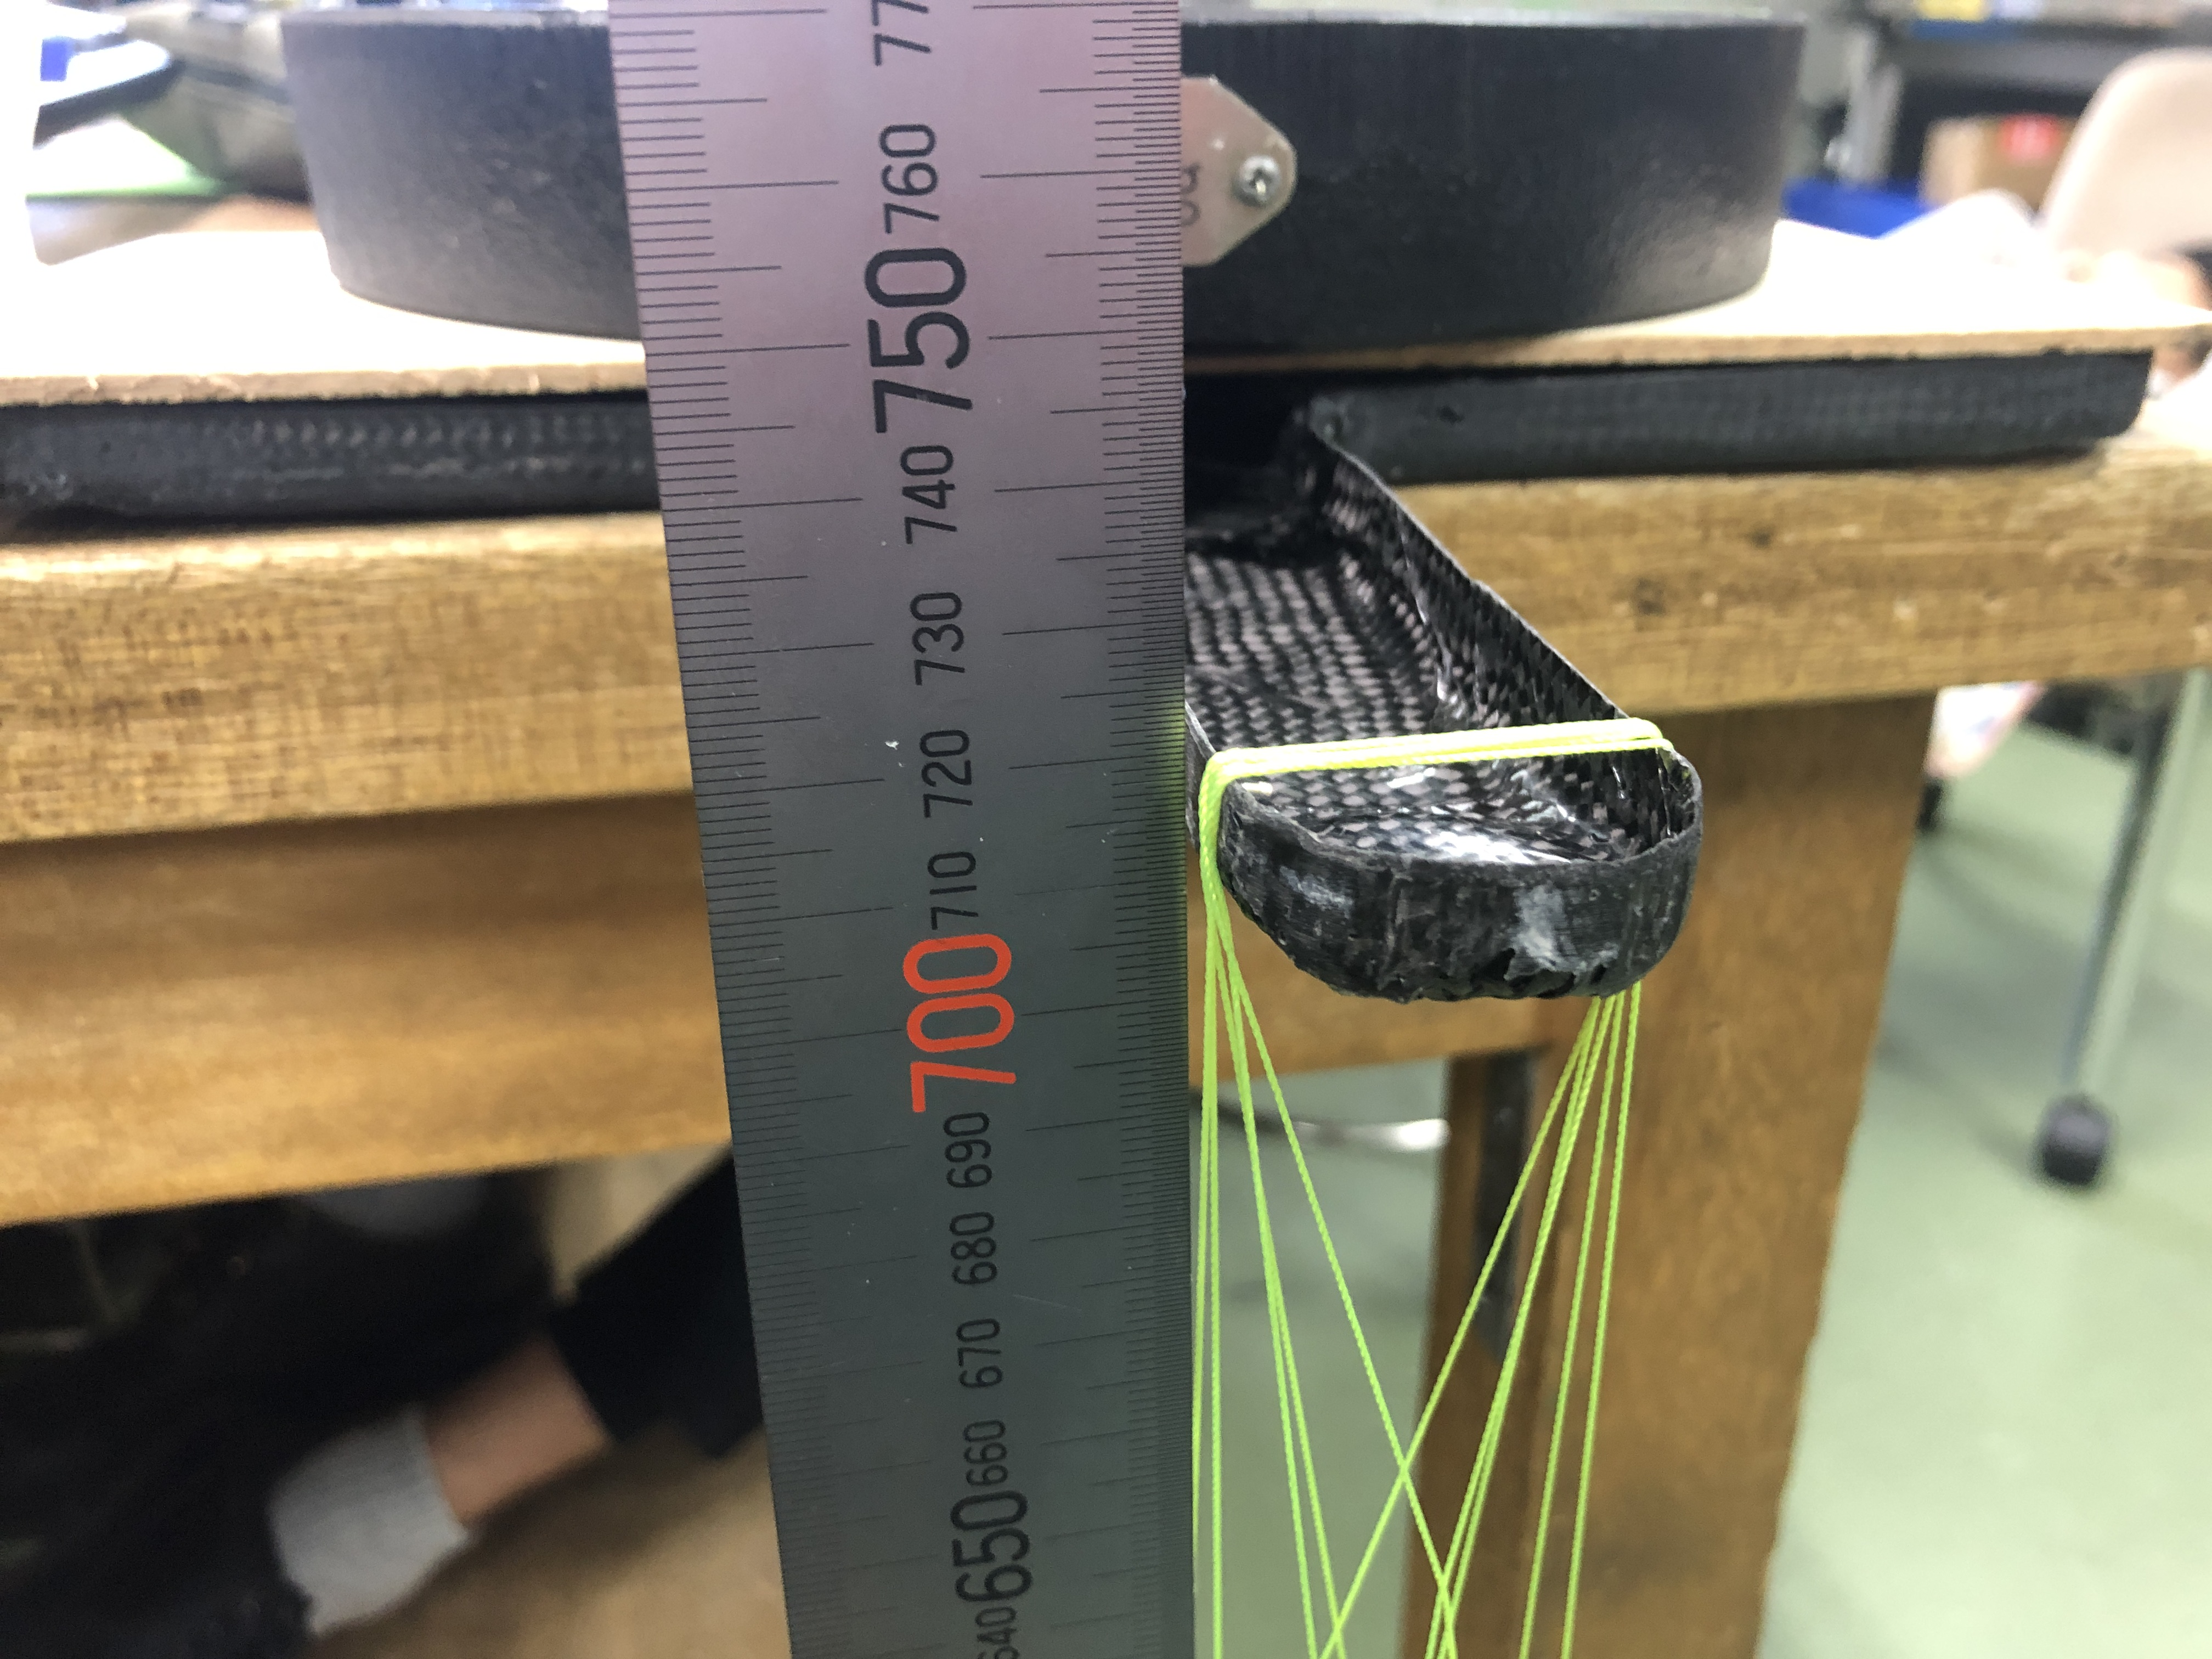
\includegraphics[width=120mm]{img/29.JPG}
    \end{center}
  \caption{たわみを計測しているフレーム}
 \label{fig:robot}
\end{figure}

\begin{figure}[htbp]
  \begin{center}
    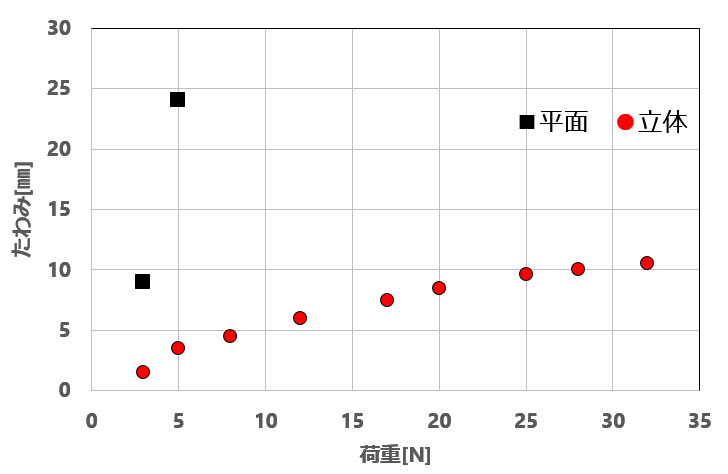
\includegraphics[width=120mm]{img/22.png}
    \end{center}
  \caption{荷重・たわみ線図}
 \label{fig:robot}
\end{figure}

\section{考察}
平面フレームから立体フレームにすることで,断面二次モーメントの値が変化する.構造物の耐久性を向上させる上で,設計上の指標として用いられる.試験結果より平面体に比べ立体の方が,断面二次モーメントが大きいため剛性が向上する.

\chapter{まとめ}
\section{結論}
平面から立体フレームにすることで,積層枚数を減らすことができより軽量で剛性のあるフレームを製作する事ができる.

\section{今後の課題}
またより厳密な質量管理を行ったフレーム製作を行うために,積層前に樹脂,カーボンクロスの質量を測っておくことでより完成後の質量を推定することで,より厳密に制作が行えるだろう.

\begin{thebibliography}{8}
\item
Fibreglass/FRP 2014/5/


https://www.youtube.com/watch?v=keBwRhkfuOQ
\item
HowToMakeYourOwnCarbonFiberParts 2008/11/20


https://www.youtube.com/watch?v=IAdVO8Rkv6c
\end{thebibliography}









\chapter*{謝辞}
\addcontentsline{toc}{chapter}{謝辞}
本論文作成にあたり研究の考え方,方法のまとめ方など長期にわたって熱意のあるご指導,ご鞭撻していただいた,伊藤恒平教授に厚く御礼申し上げます.

特に制御においても論文の書き方においても論文を何度も読んでいただき,指導していただいた伊藤恒平教授,に大変ご苦労をかけてしまいましたことにも心よりお詫び申し上げます.

その他,助けていただいた多くの皆様に心から感謝しております.ありがとうございました.


\end{document}






